\documentclass{beamer}
%\documentclass[handout]{beamer}

\pdfcompresslevel9

\usepackage{graphicx}
\usepackage{epic}
\usepackage{epsfig}
\usepackage{eepicemu}
\usepackage{color}
\usepackage{alltt}
\usepackage{cancel}
\usepackage{hhline}
\usepackage{amssymb}
\usepackage{verbatim}
\usepackage{boxedminipage}
\usepackage{listings}
\usepackage{helvet}
\usepackage{pgf}
\usepackage{tikz}
\usepackage{xspace}
\usepackage{dsfont}
\usepackage[noend]{algorithmic}
\usepackage{mathrsfs}
\usepackage{pifont}

\hypersetup{%
	pdftitle={\inserttitle},%
	pdfauthor={\insertauthor},%
	pdfsubject={},%
	pdfkeywords={}%
}

\DeclareGraphicsExtensions{.pdftex,.png,.pdf,.jpg}
\DeclareGraphicsRule{.pdftex}{pdf}{*}{}

\begin{lrbox}{2233}
\begin{picture}(0,0)
\put(300,-20){
\includegraphics[width=2cm]{satabs-small}}
\end{picture}
\end{lrbox}

\institute[]{
\includegraphics[width=3cm]{satabs-small}}

\usetheme{boxes}
\usefonttheme[stillsansseriftext,stillsansserifsmall]{serif}
\setbeamerfont{frametitle}{size=\large,series=\bfseries,shape=\sf}
\addfootbox{structure}{\,\sf{\bf \insertshorttitle} --
\href{http://www.cprover.org/}{http://www.cprover.org/}\hfill\insertframenumber\,}
\addheadbox{structure}{\usebox{2233}}

\renewcommand{\implies}{\Rightarrow}

\begingroup\makeatletter\ifx\SetFigFont\undefined%
\gdef\SetFigFont#1#2#3#4#5{%
  \reset@font\fontsize{#1}{#2pt}%
  \fontfamily{#3}\fontseries{#4}\fontshape{#5}%
  \selectfont}%
\fi\endgroup%

% COLORS

% butter (yellowish)
\definecolor{tabutter}{rgb}{0.98824, 0.91373, 0.30980}		% #fce94f
\definecolor{ta2butter}{rgb}{0.92941, 0.83137, 0}		% #edd400
\definecolor{ta3butter}{rgb}{0.76863, 0.62745, 0}		% #c4a000

% orange
\definecolor{taorange}{rgb}{0.98824, 0.68627, 0.24314}		% #fcaf3e
\definecolor{ta2orange}{rgb}{0.96078, 0.47451, 0}		% #f57900
\definecolor{ta3orange}{rgb}{0.80784, 0.36078, 0}		% #ce5c00

% chocolate (brownish)
\definecolor{tachocolate}{rgb}{0.91373, 0.72549, 0.43137}	% #e9b96e
\definecolor{ta2chocolate}{rgb}{0.75686, 0.49020, 0.066667}	% #c17d11
\definecolor{ta3chocolate}{rgb}{0.56078, 0.34902, 0.0078431}	% #8f5902

% chameleon (greenish)
\definecolor{tachameleon}{rgb}{0.54118, 0.88627, 0.20392}	% #8ae234
\definecolor{ta2chameleon}{rgb}{0.45098, 0.82353, 0.086275}	% #73d216
\definecolor{ta3chameleon}{rgb}{0.30588, 0.60392, 0.023529}	% #4e9a06

% sky blue
\definecolor{taskyblue}{rgb}{0.44706, 0.56078, 0.81176}		% #728fcf
\definecolor{ta2skyblue}{rgb}{0.20392, 0.39608, 0.64314}	% #3465a4
\definecolor{ta3skyblue}{rgb}{0.12549, 0.29020, 0.52941}	% #204a87

% plum (violettish)
\definecolor{taplum}{rgb}{0.67843, 0.49804, 0.65882}		% #ad7fa8
\definecolor{ta2plum}{rgb}{0.45882, 0.31373, 0.48235}		% #75507b
\definecolor{ta3plum}{rgb}{0.36078, 0.20784, 0.4}		% #5c3566

% scarlet red
\definecolor{tascarletred}{rgb}{0.93725, 0.16078, 0.16078}	% #ef2929
\definecolor{ta2scarletred}{rgb}{0.8, 0, 0}			% #cc0000
\definecolor{ta3scarletred}{rgb}{0.64314, 0, 0}			% #a40000

% aluminium
\definecolor{taaluminium}{rgb}{0.93333, 0.93333, 0.92549}	% #eeeeec
\definecolor{ta2aluminium}{rgb}{0.82745, 0.84314, 0.81176}	% #d3d7cf
\definecolor{ta3aluminium}{rgb}{0.72941, 0.74118, 0.71373}	% #babdb6

% gray
\definecolor{tagray}{rgb}{0.53333, 0.54118, 0.52157}		% #888a85
\definecolor{ta2gray}{rgb}{0.33333, 0.34118, 0.32549}		% #555753
\definecolor{ta3gray}{rgb}{0.18039, 0.20392, 0.21176}		% #2e3436

% gray
\definecolor{tagray}{rgb}{0.53333, 0.54118, 0.52157}		% #888a85

\usecolortheme[named=ta3skyblue]{structure}

\setbeamercolor{block body}{fg=black,bg=ta3skyblue!10}
\setbeamercolor{block title}{fg=black,bg=ta3skyblue!30}
\mode<handout>{\setbeamercolor{block body}{fg=black,bg=white!90!black}}
\mode<handout>{\setbeamercolor{block title}{fg=black,bg=white!70!black}}

\newcommand{\RETURN}{\STATE \textbf{return}~}
%\renewcommand{\ENDIF}{}

\newcommand{\power}[1]{\mathscr P({#1})}

\newcommand{\mycheck}{{\color{ta3chameleon}\ding{52}}}
\newcommand{\myfail}{{\color{ta3scarletred}\ding{56}}}


% LTL
\def\TEMPOP#1{\mathrm{\bf #1}}
\def\X{\TEMPOP{X}}
\def\F{\TEMPOP{F}}
\def\E{\TEMPOP{E}}
\def\A{\TEMPOP{A}}
\def\G{\TEMPOP{G}}
\def\U{\mathrel{\TEMPOP{U}}}
\def\R{\mathrel{\TEMPOP{R}}}

%\usepackage{circle}

\title{Predicate Abstraction with SATABS}

\date{Version 1.0, 2010}

%\usetikzlibrary{shapes}

\begin{document}

% ------------------------------------------------------------------------
% ------------------------------------------------------------------------
% ------------------------------------------------------------------------

\frame[plain]{\titlepage}

% ------------------------------------------------------------------------
% ------------------------------------------------------------------------
% ------------------------------------------------------------------------

\begin{frame}
\frametitle{Outline}
\setcounter{tocdepth}{1}
\tableofcontents
\setcounter{tocdepth}{2}
\end{frame}

% ------------------------------------------------------------------------
% ------------------------------------------------------------------------
% ------------------------------------------------------------------------

\section{Introduction}

% ------------------------------------------------------------------------
% ------------------------------------------------------------------------
% ------------------------------------------------------------------------

\begin{frame}

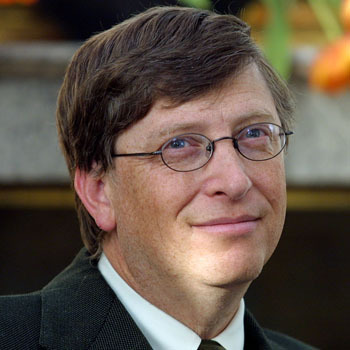
\includegraphics[width=0.2\textwidth]{bill_gates_718639}
\vfill

\begin{center}
\colorbox{tabutter!50!white}{
\begin{minipage}{0.8\textwidth}
\begin{center}
``{\it\rmfamily
Things like even software verification, this has been the Holy Grail of
computer science for many decades, but now in some very key areas, for example,
driver verification we're building tools that can do
{\bf\slshape\rmfamily actual proof} about the
software and how it works in order to guarantee the reliability.''}
\end{center}
\end{minipage}}
\end{center}
\vfill

\hfill {\footnotesize Bill Gates, April 18, 2002}\\
\hfill {\footnotesize Keynote address at WinHec 2002}

\end{frame}

% ------------------------------------------------------------------------
% ------------------------------------------------------------------------
% ------------------------------------------------------------------------

\begin{frame}

\begin{center}
\colorbox{tabutter!50!white}{
\begin{minipage}{0.9\textwidth}
\begin{center}
``{\it\rmfamily
One of the least visible ways that Microsoft Research contributed to Vista,
but something I like to talk about, is the work we did on what's called the
Static Driver Verifier.  People who develop device drivers for Vista can
verify the properties of their drivers before they ever even attempt to test
that.  What's great about this technology is there is no testing involved. 
For the properties that it is proving, they are either true or false.\\
You don't have to ask yourself \\
``{\bf\slshape\rmfamily
Did I come up with a good test case or not?}''}
\end{center}
\end{minipage}}
\end{center}
\vfill

\hfill {\footnotesize Rick Rashid, Microsoft Research chief}\\
\hfill {\footnotesize father of CMU's Mach Operating System (Mac~OS~X)}\\
\hfill {\footnotesize news.cnet.com interview, 2008}

\end{frame}

% ------------------------------------------------------------------------
% ------------------------------------------------------------------------
% ------------------------------------------------------------------------

\begin{frame}
\frametitle{Model Checking with Predicate Abstraction}

\begin{itemize}

\item A \alert{heavy-weight} formal analysis technique
\vfill

\item Recent successes in software verification,\\
e.g., SLAM at Microsoft
\vfill

\item The abstraction reduces the size of the model\\
by {\color{ta3chameleon}removing irrelevant detail}

\end{itemize}

\end{frame}

% ------------------------------------------------------------------------
% ------------------------------------------------------------------------
% ------------------------------------------------------------------------

\begin{frame}
\frametitle{Model Checking with Predicate Abstraction}

\begin{itemize}

\item Goal: make the abstract model
{\color{ta3chameleon}small enough} for
an analysis with a BDD-based Model Checker
\vfill

\item Idea: {\color{ta3chameleon}only track predicates on data},\\
and remove data variables from model
\vfill

\item Mostly works with \alert{control-flow dominated properties}

\end{itemize}

\end{frame}

% ------------------------------------------------------------------------
% ------------------------------------------------------------------------
% ------------------------------------------------------------------------

\subsection{Notation for Abstractions}

\begin{frame}
\frametitle{Notation for Abstractions}

\begin{center}
\begin{minipage}{0.8\textwidth}
\begin{block}{\centering Abstract Domain}
\vspace{0.5ex}
\centering Approximate representation of \\
\emph{\color{ta3chameleon}sets of concrete values}
\vspace{0.5ex}
\end{block}
\end{minipage}

\[ \scalebox{1.5}{$\mbox{\Large $S$} \begin{array}{c}
\alpha \\[-1ex]
\longrightarrow \\
\longleftarrow \\[-1ex]
\gamma
\end{array} \mbox{\Large $\hat S$}$} \]

\end{center}

\end{frame}

% ------------------------------------------------------------------------
% ------------------------------------------------------------------------
% ------------------------------------------------------------------------

\subsection{Predicate Abstraction as Abstract Domain}

\begin{frame}
\frametitle{Predicate Abstraction as Abstract Domain}

\begin{itemize}
\item We are given a set of predicates over $S$,\\
denoted by $\Pi_1,\ldots,\Pi_n$.
\vfill

\item An abstract state is a valuation of the predicates:
%
\[ \hat S = \mathbb B ^ n \]
\vfill

\item The abstraction function:
%
\[ \alpha(s) = \langle \Pi_1(s), \ldots, \Pi_n(s) \rangle \]
\end{itemize}

\end{frame}

% ------------------------------------------------------------------------
% ------------------------------------------------------------------------
% ------------------------------------------------------------------------

\subsection{Example}

\definecolor{absstate}{rgb}{.6,.8,1}

\newlength{\sdist}
\setlength{\sdist}{2.2cm}

\newcommand{\slabel}[1]{\begin{picture}(0,0)
\put(0,-2.5){\makebox[0cm][c]{$\begin{array}{c}#1\end{array}$}}
\end{picture}}

\begin{frame}
\frametitle{Predicate Abstraction: the Basic Idea}

Concrete states over variables $x$, $y$:

\begin{center}
\begin{tikzpicture}
\onslide<3->{
  \fill[color=absstate] (-.4\sdist,-.4\sdist) rectangle ( .4\sdist,1.4\sdist);
  \fill[color=absstate] ( .6\sdist,-.4\sdist) rectangle (2.4\sdist, .4\sdist);
  \fill[color=absstate] ( .6\sdist, .6\sdist) rectangle (1.4\sdist,1.4\sdist);
  \fill[color=absstate] (1.6\sdist, .6\sdist) rectangle (2.4\sdist,1.4\sdist);
}
%
\tikzstyle{state}=
  [circle,thick,draw=black,
   fill=tabutter,minimum size=13mm]
\draw (0\sdist,0\sdist) node[state] (s00) {\slabel{x=1\\y=0}};
\draw (1\sdist,0\sdist) node[state] (s10) {\slabel{x=1\\y=1}};
\draw (2\sdist,0\sdist) node[state] (s20) {\slabel{x=1\\y=2}};
\draw (0\sdist,1\sdist) node[state] (s01) {\slabel{x=2\\y=0}};
\draw (1\sdist,1\sdist) node[state] (s11) {\slabel{x=2\\y=1}};
\draw (2\sdist,1\sdist) node[state] (s21) {\slabel{x=0\\y=0}};
\draw[->,very thick] (s01) -- (s11);
\draw[->,very thick] (s00) -- (s10);
\draw[->,very thick] (s10) -- (s20);
\draw[->,very thick] (s01)+(-.35\sdist,.35\sdist)
                     .. controls +(150:.55\sdist) .. (s01);
\draw[->,very thick] (s11) .. controls +(20:.7\sdist) and +(70:.7\sdist)
                           .. (s11);
\pause\pause
\draw (0\sdist,.5\sdist) node {\alert{\Large $p_1,p_2$}};
\draw (1.5\sdist,-.4\sdist) node {\alert{\Large $\neg p_1,\neg p_2$}};
\draw (1\sdist,.6\sdist) node {\alert{\Large $p_1,\neg p_2$}};
\draw (2\sdist,.6\sdist) node {\alert{\Large $\neg p_1,p_2$}};
\end{tikzpicture}
\end{center}

\onslide<2->{
\begin{minipage}{.4\textwidth}
Predicates:\\
\hspace*{1cm}{\large $p_1 \iff x>y$}\\
\hspace*{1cm}{\large $p_2 \iff y=0$}
\end{minipage}}
\hfill
\onslide<4->{\Large Abstract Transitions?}

\end{frame}

% ------------------------------------------------------------------------
% ------------------------------------------------------------------------
% ------------------------------------------------------------------------

\section{Existential Abstraction}

\begin{frame}
\frametitle{Existential
Abstraction\footnote{Clarke, Grumberg, Long: {\it Model Checking and Abstraction},
ACM~TOPLAS, 1994}}

\begin{definition}[Existential Abstraction]
A model $\hat M=( \hat S, \hat S_0, \hat T)$ is an
\emph{\alert{existential abstraction}} of $M=( S, S_0, T)$ with
respect to $\alpha: S \rightarrow \hat S$ iff
%
\begin{itemize}
\item $\exists s \in S_0.\, \alpha(s)=\hat s \quad \implies\quad \hat s \in \hat
S_0$ \quad and
\item $\exists (s,s') \in T.\, \alpha(s)=\hat s \land \alpha(s')=\hat s'
\quad\implies\quad (\hat s, \hat s') \in \hat T$.
\end{itemize}
\end{definition}

\end{frame}

% ------------------------------------------------------------------------
% ------------------------------------------------------------------------
% ------------------------------------------------------------------------

\begin{frame}
\frametitle{Minimal Existential Abstractions}

There are obviously many choices for an existential abstraction
for a given $\alpha$.
\vfill

\begin{definition}[Minimal Existential Abstraction]
A model $\hat M=( \hat S, \hat S_0, \hat T)$ is the
\emph{\alert{minimal existential abstraction}} of $M=( S, S_0, T)$ with
respect to $\alpha: S \rightarrow \hat S$ iff
%
\begin{itemize}
\item $\exists s \in S_0.\, \alpha(s)=\hat s \quad \iff \quad \hat s \in \hat
S_0$ \quad and
\item $\exists (s,s') \in T.\, \alpha(s)=\hat s \land \alpha(s')=\hat s'
\quad\iff \quad (\hat s, \hat s') \in \hat T$.
\end{itemize}
\end{definition}
\vfill

This is the most precise existential abstraction.

\end{frame}

% ------------------------------------------------------------------------
% ------------------------------------------------------------------------
% ------------------------------------------------------------------------

\begin{frame}
\frametitle{Existential Abstraction}

We write $\alpha(\pi)$ for the abstraction of a path $\pi=s_0,s_1,\ldots$:
%
\[ \alpha(\pi) \,=\, \alpha(s_0), \alpha(s_1), \ldots \]
\vfill
\pause

\begin{lemma}
Let $\hat M$ be an existential abstraction of $M$.
The abstraction of every path (trace) $\pi$ in $M$ is a path
(trace) in $\hat M$.
\[ \pi \in M \quad\implies\quad \alpha(\pi) \in \hat M \]
\end{lemma}

Proof by induction.

We say that $\hat M$ \alert{overapproximates} $M$.

\end{frame}

% ------------------------------------------------------------------------
% ------------------------------------------------------------------------
% ------------------------------------------------------------------------

\begin{frame}
\frametitle{Abstracting Properties}

Reminder: we are using
%
\begin{itemize}
\item a set of \alert{atomic propositions} (predicates) $A$, and
\item a \alert{state-labelling function} $L : S \rightarrow \ \power{A}$
\end{itemize}
%
in order to define the meaning of propositions in our properties.

\end{frame}

% ------------------------------------------------------------------------
% ------------------------------------------------------------------------
% ------------------------------------------------------------------------

\begin{frame}
\frametitle{Abstracting Properties}

We define an abstract version of it as follows:

\begin{itemize}
\item First of all, the negations are pushed into the atomic propositions.

E.g., we will have
\[ x=0 \quad \in A \]
\alert{and}
\[ x\not =0 \quad \in A \]

\end{itemize}

\end{frame}

% ------------------------------------------------------------------------
% ------------------------------------------------------------------------
% ------------------------------------------------------------------------

\begin{frame}
\frametitle{Abstracting Properties}

\begin{itemize}

\item
An abstract state $\hat s$ is labelled with $a \in A$ iff
\alert{all} of the corresponding concrete states are labelled with $a$.
%
\[ a \in \hat L(\hat s) \quad\iff\quad \forall s | \alpha(s)=\hat s.\, a \in L(s) \]
\vfill

\item This also means that an abstract state may have neither the label
$x=0$ nor the label $x\not =0$ -- this may happen if it concretizes to
concrete states with different labels!

\end{itemize}

\end{frame}

% ------------------------------------------------------------------------
% ------------------------------------------------------------------------
% ------------------------------------------------------------------------

\begin{frame}
\frametitle{Conservative Abstraction}

The keystone is that existential abstraction is \alert{conservative}
for certain properties:
%
\begin{theorem}[Clarke/Grumberg/Long 1994]
Let $\phi$ be a $\forall$CTL* formula where all negations
are pushed into the atomic propositions, and let $\hat M$
be an existential abstraction of $M$. If $\phi$ holds on
$\hat M$, then it also holds on $M$.
\[ \hat M \models \phi \quad\implies\quad M \models \phi \]
\end{theorem}
%
We say that an existential abstraction is conservative for $\forall$CTL*
properties. {\color{ta3skyblue}The same result can be obtained
for LTL properties}.
\vfill

The proof uses the lemma and is by induction on the structure of
$\phi$. The converse usually does not hold.
\end{frame}

% ------------------------------------------------------------------------
% ------------------------------------------------------------------------
% ------------------------------------------------------------------------

\begin{frame}
\frametitle{Conservative Abstraction}

We hope: computing $\hat M$ and checking $\hat M \models \phi$ is easier
than checking $M \models \phi$.

\end{frame}

% ------------------------------------------------------------------------
% ------------------------------------------------------------------------
% ------------------------------------------------------------------------

\begin{frame}
\frametitle{Back to the Example}

\begin{center}
\begin{tikzpicture}
\onslide<1->{
  \fill[color=absstate] (-.4\sdist,-.4\sdist) rectangle ( .4\sdist,1.4\sdist);
  \fill[color=absstate] ( .6\sdist,-.4\sdist) rectangle (2.4\sdist, .4\sdist);
  \fill[color=absstate] ( .6\sdist, .6\sdist) rectangle (1.4\sdist,1.4\sdist);
  \fill[color=absstate] (1.6\sdist, .6\sdist) rectangle (2.4\sdist,1.4\sdist);
}
%
\tikzstyle{state}=
  [circle,thick,draw=black,
   fill=tabutter,minimum size=13mm]
\draw (0\sdist,0\sdist) node[state] (s00) {\slabel{x=1\\y=0}};
\draw (1\sdist,0\sdist) node[state] (s10) {\slabel{x=1\\y=1}};
\draw (2\sdist,0\sdist) node[state] (s20) {\slabel{x=1\\y=2}};
\draw (0\sdist,1\sdist) node[state] (s01) {\slabel{x=2\\y=0}};
\draw (1\sdist,1\sdist) node[state] (s11) {\slabel{x=2\\y=1}};
\draw (2\sdist,1\sdist) node[state] (s21) {\slabel{x=0\\y=0}};
\draw[->,very thick] (s01) -- (s11);
\draw[->,very thick] (s00) -- (s10);
\draw[->,very thick] (s10) -- (s20);
\draw[->,very thick] (s01)+(-.35\sdist,.35\sdist)
                     .. controls +(150:.55\sdist) .. (s01);
\draw[->,very thick] (s11) .. controls +(20:.7\sdist) and +(70:.7\sdist)
                           .. (s11);
%
\draw (0\sdist,.5\sdist) node {\alert{\Large $p_1,p_2$}};
\draw (1.5\sdist,-.4\sdist) node {\alert{\Large $\neg p_1,\neg p_2$}};
\draw (1\sdist,.6\sdist) node {\alert{\Large $p_1,\neg p_2$}};
\draw (2\sdist,.6\sdist) node {\alert{\Large $\neg p_1,p_2$}};
%
\pause
%
\tikzstyle{abstran}=[->,line width=.12cm,color=ta3skyblue]
\draw[abstran] (-.8\sdist,.5\sdist) -- (-.4\sdist,.5\sdist);
\pause
\draw[abstran] (.35\sdist,1.2\sdist) -- (.65\sdist,1.2\sdist);
\pause
\draw[abstran] (.35\sdist,.2\sdist)  -- (.65\sdist,.2\sdist);
\pause
\draw[abstran] (1.3\sdist,1.1\sdist) .. controls +(20:.7\sdist) and +(70:.7\sdist)
            .. (1.1\sdist,1.3\sdist);
\pause
\draw[abstran] (2.3\sdist,.1\sdist) .. controls +(20:.7\sdist) and +(70:.7\sdist)
            .. (2.1\sdist,.3\sdist);
\end{tikzpicture}
\end{center}

\end{frame}

% ------------------------------------------------------------------------
% ------------------------------------------------------------------------
% ------------------------------------------------------------------------

\begin{frame}
\frametitle{Let's try a Property}

\vspace*{-1cm}
\begin{center}
\begin{tikzpicture}
\onslide<1->{
  \fill[color=absstate] (-.4\sdist,-.4\sdist) rectangle ( .4\sdist,1.4\sdist);
  \fill[color=absstate] ( .6\sdist,-.4\sdist) rectangle (2.4\sdist, .4\sdist);
  \fill[color=absstate] ( .6\sdist, .6\sdist) rectangle (1.4\sdist,1.4\sdist);
  \fill[color=absstate] (1.6\sdist, .6\sdist) rectangle (2.4\sdist,1.4\sdist);
}
%
\tikzstyle{state}=
  [circle,thick,draw=black,
   fill=tabutter,minimum size=13mm]
\draw (0\sdist,0\sdist) node[state] (s00) {\slabel{x=1\\y=0}};
\draw (1\sdist,0\sdist) node[state] (s10) {\slabel{x=1\\y=1}};
\draw (2\sdist,0\sdist) node[state] (s20) {\slabel{x=1\\y=2}};
\draw (0\sdist,1\sdist) node[state] (s01) {\slabel{x=2\\y=0}};
\draw (1\sdist,1\sdist) node[state] (s11) {\slabel{x=2\\y=1}};
\draw (2\sdist,1\sdist) node[state] (s21) {\slabel{x=0\\y=0}};
\draw[->,very thick] (s01) -- (s11);
\draw[->,very thick] (s00) -- (s10);
\draw[->,very thick] (s10) -- (s20);
\draw[->,very thick] (s01)+(-.35\sdist,.35\sdist)
                     .. controls +(150:.55\sdist) .. (s01);
\draw[->,very thick] (s11) .. controls +(20:.7\sdist) and +(70:.7\sdist)
                           .. (s11);
%
\draw (0\sdist,.5\sdist) node {\alert{\Large $p_1,p_2$}};
\draw (1.5\sdist,-.4\sdist) node {\alert{\Large $\neg p_1,\neg p_2$}};
\draw (1\sdist,.6\sdist) node {\alert{\Large $p_1,\neg p_2$}};
\draw (2\sdist,.6\sdist) node {\alert{\Large $\neg p_1,p_2$}};
%
\tikzstyle{abstran}=[->,line width=.12cm,color=ta3skyblue]
\draw[abstran] (-.8\sdist,.5\sdist) -- (-.4\sdist,.5\sdist);
\draw[abstran] (.35\sdist,1.2\sdist) -- (.65\sdist,1.2\sdist);
\draw[abstran] (.35\sdist,.2\sdist)  -- (.65\sdist,.2\sdist);
\draw[abstran] (1.3\sdist,1.1\sdist) .. controls +(20:.7\sdist) and +(70:.7\sdist)
            .. (1.1\sdist,1.3\sdist);
\draw[abstran] (2.3\sdist,.1\sdist) .. controls +(20:.7\sdist) and +(70:.7\sdist)
            .. (2.1\sdist,.3\sdist);
\pause
\draw (.3\sdist,1.4\sdist) node {\huge \mycheck};
\draw (.9\sdist,1.4\sdist) node {\huge \mycheck};
\draw (1.4\sdist,.4\sdist) node {\huge \mycheck};
\end{tikzpicture}
\end{center}

\vfill

Property:\\
\qquad$x>y \vee y\not=0 \quad \iff\quad p_1\vee \neg p_2$

\end{frame}

% ------------------------------------------------------------------------
% ------------------------------------------------------------------------
% ------------------------------------------------------------------------

\begin{frame}
\frametitle{Another Property}

\vspace*{-1cm}
\begin{center}
\begin{tikzpicture}
\onslide<1->{
  \fill[color=absstate] (-.4\sdist,-.4\sdist) rectangle ( .4\sdist,1.4\sdist);
  \fill[color=absstate] ( .6\sdist,-.4\sdist) rectangle (2.4\sdist, .4\sdist);
  \fill[color=absstate] ( .6\sdist, .6\sdist) rectangle (1.4\sdist,1.4\sdist);
  \fill[color=absstate] (1.6\sdist, .6\sdist) rectangle (2.4\sdist,1.4\sdist);
}
%
\onslide<3->{
  \fill[color=tascarletred!30!white] ( .6\sdist,-.4\sdist) rectangle (2.4\sdist, .4\sdist);
}
%
\tikzstyle{state}=
  [circle,thick,draw=black,
   fill=tabutter,minimum size=13mm]
\draw (0\sdist,0\sdist) node[state] (s00) {\slabel{x=1\\y=0}};
\draw (1\sdist,0\sdist) node[state] (s10) {\slabel{x=1\\y=1}};
\draw (2\sdist,0\sdist) node[state] (s20) {\slabel{x=1\\y=2}};
\draw (0\sdist,1\sdist) node[state] (s01) {\slabel{x=2\\y=0}};
\draw (1\sdist,1\sdist) node[state] (s11) {\slabel{x=2\\y=1}};
\draw (2\sdist,1\sdist) node[state] (s21) {\slabel{x=0\\y=0}};
\draw[->,very thick] (s01) -- (s11);
\draw[->,very thick] (s00) -- (s10);
\draw[->,very thick] (s10) -- (s20);
\draw[->,very thick] (s01)+(-.35\sdist,.35\sdist)
                     .. controls +(150:.55\sdist) .. (s01);
\draw[->,very thick] (s11) .. controls +(20:.7\sdist) and +(70:.7\sdist)
                           .. (s11);
%
\draw (0\sdist,.5\sdist) node {\alert{\Large $p_1,p_2$}};
\draw (1.5\sdist,-.4\sdist) node {\alert{\Large $\neg p_1,\neg p_2$}};
\draw (1\sdist,.6\sdist) node {\alert{\Large $p_1,\neg p_2$}};
\draw (2\sdist,.6\sdist) node {\alert{\Large $\neg p_1,p_2$}};
%
\tikzstyle{abstran}=[->,line width=.12cm,color=ta3skyblue]
\draw[abstran] (-.8\sdist,.5\sdist) -- (-.4\sdist,.5\sdist);
\draw[abstran] (.35\sdist,1.2\sdist) -- (.65\sdist,1.2\sdist);
\draw[abstran] (.35\sdist,.2\sdist)  -- (.65\sdist,.2\sdist);
\draw[abstran] (1.3\sdist,1.1\sdist) .. controls +(20:.7\sdist) and +(70:.7\sdist)
            .. (1.1\sdist,1.3\sdist);
\draw[abstran] (2.3\sdist,.1\sdist) .. controls +(20:.7\sdist) and +(70:.7\sdist)
            .. (2.1\sdist,.3\sdist);
\pause
\draw (.3\sdist,1.4\sdist) node {\huge \mycheck};
\draw (.9\sdist,1.4\sdist) node {\huge \mycheck};
\pause
\draw (1.4\sdist,.4\sdist) node {\huge \myfail};
\end{tikzpicture}
\end{center}

\vfill

\begin{minipage}{.3\textwidth}
Property:\\
\qquad$x>y \quad \iff\quad p_1$
\end{minipage}
\hfill{\onslide<4->{\colorbox{ta3butter!30!white}{But: the counterexample is
\alert{spurious}}}}

\end{frame}

% ------------------------------------------------------------------------
% ------------------------------------------------------------------------
% ------------------------------------------------------------------------

\section{Predicate Abstraction for Software}

\subsection{SLAM}

\begin{frame}
\frametitle{SLAM}
\begin{itemize}
\item Microsoft blames most Windows crashes on
\alert{third party device drivers}
\vfill

\item The Windows device driver API is quite complicated
\vfill

\item Drivers are low level C code
\vfill

\item SLAM: Tool to automatically check
device drivers for certain errors
\vfill

\item SLAM is shipped with Device Driver Development Kit
\vfill

\item Full detail available at
\url{http://research.microsoft.com/slam/}
\end{itemize}

\end{frame}

% ------------------------------------------------------------------------
% ------------------------------------------------------------------------
% ------------------------------------------------------------------------

\subsection{SLIC}

\begin{frame}
\frametitle{SLIC}

\begin{itemize}
\item {\color{ta3skyblue}Finite state language} for defining properties

\begin{itemize}
\item Monitors behavior of C code
\item Temporal safety properties (security automata)
\item familiar C syntax
\end{itemize}
\vfill

\item Suitable for expressing control-dominated properties
\begin{itemize}
\item e.g., proper sequence of events
\item can track data values
\end{itemize}

\end{itemize}

\end{frame}

% ------------------------------------------------------------------------
% ------------------------------------------------------------------------
% ------------------------------------------------------------------------

\begin{frame}[fragile]
\frametitle{SLIC Example}

\begin{columns}
\begin{column}{.5\textwidth}
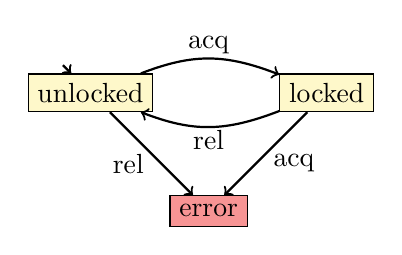
\begin{tikzpicture}
\tikzstyle{state}=[rectangle,draw=black,fill=tabutter!30!white]
\draw (0,2) node[state] (unlocked) {unlocked};
\draw (3,2) node[state] (locked) {locked};
\draw[->,thick] (unlocked) .. controls (1.3,2.5) and (1.7,2.5) .. (locked);
\draw[->,thick] (locked) .. controls (1.7,1.5) and (1.3,1.5) .. (unlocked);
\draw (1.5,2.6) node {acq};
\draw (1.5,1.4) node {rel};
\draw[->,thick] (unlocked)+(-.35\sdist,.35\sdist) -- (unlocked);
\pause
\draw (1.5,0.5) node[state,fill=tascarletred!50!white] (error) {error};
\draw[->,thick] (locked) -- (error);
\draw[->,thick] (unlocked) -- (error);
\draw (.8,1.1) node[left] {rel};
\draw (2.2,1.1) node[right] {acq};
\end{tikzpicture}
\end{column}
\begin{column}{.5\textwidth}
\begin{lstlisting}[language=C,basicstyle=\small,morekeywords={abort,state,entry}]
state {
  enum {Locked,Unlocked}  
    s = Unlocked;
}

KeAcquireSpinLock.entry {
  if (s==Locked) abort;
  else s = Locked;
}

KeReleaseSpinLock.entry {
  if (s==Unlocked) abort;
  else s = Unlocked;
}
\end{lstlisting}
\end{column}
\end{columns}

\end{frame}

% ------------------------------------------------------------------------
% ------------------------------------------------------------------------
% ------------------------------------------------------------------------

\subsection{Refinement Example}

\newlength{\vdist}
\setlength{\vdist}{3.1ex}
\newlength{\hdist}
\setlength{\hdist}{.7cm}

\lstset{language=C,basicstyle=\small,escapechar=@}

\begin{frame}[fragile]
\frametitle{Refinement Example}

\begin{tikzpicture}
%
\draw (5\hdist, 14.5\vdist) node[right] {\lstinline!do {!};
\draw (6\hdist, 13.5\vdist) node[right] {{\color{ta3skyblue}KeAcquireSpinLock}\lstinline!();!};
\draw (6\hdist, 12.5\vdist) node[right] {\lstinline!nPacketsOld = nPackets;!};
\draw (6\hdist, 11.5\vdist) node[right] {\lstinline!if(request) {!};
\draw (7\hdist, 10.5\vdist) node[right] {\lstinline!request = request->Next;!};
\draw (7\hdist,  9.5\vdist) node[right] {{\color{ta3skyblue}KeReleaseSpinLock}\lstinline!();!};
\draw (7\hdist,  8.5\vdist) node[right] {\lstinline!nPackets++;!};
\draw (6\hdist,  7.5\vdist) node[right] {\lstinline@}@};
\draw (5\hdist,  6.5\vdist) node[right] {\lstinline@} while(nPackets != nPacketsOld);@};
\draw (5\hdist,  4.5\vdist) node[right] {{\color{ta3skyblue}KeReleaseSpinLock}\lstinline!();!};
%
\onslide<2->{
\draw (1\hdist,10\vdist) node {
\includegraphics[width=5\hdist]{images/note}};
\draw (1\hdist,10\vdist) node
  {\begin{minipage}{4\hdist}
    \begin{center}Does this code obey the locking rule?%
    \end{center}\end{minipage}};
}
\end{tikzpicture}

\end{frame}

% ------------------------------------------------------------------------
% ------------------------------------------------------------------------
% ------------------------------------------------------------------------

\begin{frame}[fragile]
\frametitle{Refinement Example}

\begin{tikzpicture}
\tikzstyle{state}=[circle,draw=black,fill=tabutter!30!white,minimum size=.45cm]
%
\draw (5\hdist, 14.5\vdist) node[right] {\lstinline!do {!};
\draw (6\hdist, 13.5\vdist) node[right] {{\color{ta3skyblue}KeAcquireSpinLock}\lstinline!();!};
\draw (6\hdist, 11.5\vdist) node[right] {\lstinline!if(*) {!};
\draw (7\hdist,  9.5\vdist) node[right] {{\color{ta3skyblue}KeReleaseSpinLock}\lstinline!();!};
\draw (6\hdist,  7.5\vdist) node[right] {\lstinline@}@};
\draw (5\hdist,  6.5\vdist) node[right] {\lstinline@} while(*);@};
\draw (5\hdist,  4.5\vdist) node[right] {{\color{ta3skyblue}KeReleaseSpinLock}\lstinline!();!};
%
\onslide<2->{
\draw (2\hdist,  14\vdist) node[state] (l1)  {\slabel{U}};
\draw (2\hdist,  13\vdist) node[state] (l2)  {\slabel{L}};
\draw (2\hdist,  12\vdist) node[state] (l3)  {\slabel{L}};
\draw (3\hdist,  10\vdist) node[state] (l4)  {\slabel{L}};
\draw (3\hdist,   9\vdist) node[state] (l5)  {\slabel{U}};
\draw (3\hdist,   7\vdist) node[state] (l6)  {\slabel{U}};
\draw (2.5\hdist, 5\vdist) node[state] (l7)  {\slabel{U}};
\draw (2.5\hdist, 4\vdist) node[state,fill=tascarletred!70!white] (l8)  {\slabel{E}};
\draw (1\hdist,   7\vdist) node[state] (l9)  {\slabel{L}};
\draw (1.5\hdist, 5\vdist) node[state] (l10) {\slabel{L}};
\draw (1.5\hdist, 4\vdist) node[state] (l11) {\slabel{U}};
%
\draw[->] (2\hdist,14.5\vdist) -- (l1);
\draw[->] (l1) -- (l2);
\draw[->] (l2) -- (l3);
\draw[->] (l3) -- (l4);
\draw[->] (l4) -- (l5);
\draw[->] (l5) -- (l6);
\draw[->] (l6) -- (l7);
\draw[->] (l7) -- (l8);
\draw[->] (l3) -- (l9);
\draw[->] (l9) -- (l10);
\draw[->] (l10) -- (l11);
}
\onslide<3->{
\draw (2\hdist,  14\vdist) node[state,thick] (l1)  {\slabel{U}};
\draw (2\hdist,  13\vdist) node[state,thick] (l2)  {\slabel{L}};
\draw (2\hdist,  12\vdist) node[state,thick] (l3)  {\slabel{L}};
\draw (3\hdist,  10\vdist) node[state,thick] (l4)  {\slabel{L}};
\draw (3\hdist,   9\vdist) node[state,thick] (l5)  {\slabel{U}};
\draw (3\hdist,   7\vdist) node[state,thick] (l6)  {\slabel{U}};
\draw (2.5\hdist, 5\vdist) node[state,thick] (l7)  {\slabel{U}};
\draw (2.5\hdist, 4\vdist) node[state,fill=tascarletred!70!white,thick] (l8)  {\slabel{E}};
%
\draw[->,thick,color=tascarletred] (2\hdist,14.5\vdist) -- (l1);
\draw[->,thick,color=tascarletred] (l1) -- (l2);
\draw[->,thick,color=tascarletred] (l2) -- (l3);
\draw[->,thick,color=tascarletred] (l3) -- (l4);
\draw[->,thick,color=tascarletred] (l4) -- (l5);
\draw[->,thick,color=tascarletred] (l5) -- (l6);
\draw[->,thick,color=tascarletred] (l6) -- (l7);
\draw[->,thick,color=tascarletred] (l7) -- (l8);
}
\onslide<4->{
\draw (13.5\hdist,4.5\vdist) node {
\includegraphics[width=5\hdist,height=3\vdist]{images/note}};
\draw (13.5\hdist,4.5\vdist) node
  {\begin{minipage}{4\hdist}
    \begin{center}Is this path concretizable?%
    \end{center}\end{minipage}};
}
\end{tikzpicture}

\end{frame}

% ------------------------------------------------------------------------
% ------------------------------------------------------------------------
% ------------------------------------------------------------------------

\begin{frame}[fragile]
\frametitle{Refinement Example}

\begin{tikzpicture}
\tikzstyle{state}=[circle,draw=black,fill=tabutter!30!white,minimum size=.45cm]
%
\draw (5\hdist, 14.5\vdist) node[right] {\lstinline!do {!};
\draw (6\hdist, 13.5\vdist) node[right] {{\color{ta3skyblue}KeAcquireSpinLock}\lstinline!();!};
\draw (6\hdist, 12.5\vdist) node[right] {\lstinline!nPacketsOld = nPackets;!};
\draw (6\hdist, 11.5\vdist) node[right] {\lstinline!if(request) {!};
\draw (7\hdist, 10.5\vdist) node[right] {\lstinline!request = request->Next;!};
\draw (7\hdist,  9.5\vdist) node[right] {{\color{ta3skyblue}KeReleaseSpinLock}\lstinline!();!};
\draw (7\hdist,  8.5\vdist) node[right] {\lstinline!nPackets++;!};
\draw (6\hdist,  7.5\vdist) node[right] {\lstinline@}@};
\draw (5\hdist,  6.5\vdist) node[right] {\lstinline@} while(nPackets != nPacketsOld);@};
\draw (5\hdist,  4.5\vdist) node[right] {{\color{ta3skyblue}KeReleaseSpinLock}\lstinline!();!};
%
\draw (2\hdist,  14\vdist) node[state] (l1)  {\slabel{U}};
\draw (2\hdist,  13\vdist) node[state] (l2)  {\slabel{L}};
\draw (2\hdist,  12\vdist) node[state] (l3)  {\slabel{L}};
\draw (3\hdist,  10\vdist) node[state] (l4)  {\slabel{L}};
\draw (3\hdist,   9\vdist) node[state] (l5)  {\slabel{U}};
\draw (3\hdist,   7\vdist) node[state] (l6)  {\slabel{U}};
\draw (2.5\hdist, 5\vdist) node[state] (l7)  {\slabel{U}};
\draw (2.5\hdist, 4\vdist) node[state,fill=tascarletred!70!white] (l8)  {\slabel{E}};
\draw (1\hdist,   7\vdist) node[state] (l9)  {\slabel{L}};
\draw (1.5\hdist, 5\vdist) node[state] (l10) {\slabel{L}};
\draw (1.5\hdist, 4\vdist) node[state] (l11) {\slabel{U}};
%
\draw[->] (l3) -- (l9);
\draw[->] (l9) -- (l10);
\draw[->] (l10) -- (l11);
%
\draw (2\hdist,  14\vdist) node[state,thick] (l1)  {\slabel{U}};
\draw (2\hdist,  13\vdist) node[state,thick] (l2)  {\slabel{L}};
\draw (2\hdist,  12\vdist) node[state,thick] (l3)  {\slabel{L}};
\draw (3\hdist,  10\vdist) node[state,thick] (l4)  {\slabel{L}};
\draw (3\hdist,   9\vdist) node[state,thick] (l5)  {\slabel{U}};
\draw (3\hdist,   7\vdist) node[state,thick] (l6)  {\slabel{U}};
\draw (2.5\hdist, 5\vdist) node[state,thick] (l7)  {\slabel{U}};
\draw (2.5\hdist, 4\vdist) node[state,fill=tascarletred!70!white,thick] (l8)  {\slabel{E}};
%
\draw[->,thick,color=tascarletred] (2\hdist,14.5\vdist) -- (l1);
\draw[->,thick,color=tascarletred] (l1) -- (l2);
\draw[->,thick,color=tascarletred] (l2) -- (l3);
\draw[->,thick,color=tascarletred] (l3) -- (l4);
\draw[->,thick,color=tascarletred] (l4) -- (l5);
\draw[->,thick,color=tascarletred] (l5) -- (l6);
\draw[->,thick,color=tascarletred] (l6) -- (l7);
\draw[->,thick,color=tascarletred] (l7) -- (l8);
%
\onslide<2>{
\draw (13.5\hdist,4.5\vdist) node {
\includegraphics[width=5\hdist,height=3\vdist]{images/note}};
\draw (13.5\hdist,4.5\vdist) node
  {\begin{minipage}{4\hdist}
    \begin{center}This path is \alert{spurious}!%
    \end{center}\end{minipage}};
}
\onslide<3->{
\draw (14\hdist,4.5\vdist) node {
\includegraphics[width=6.5\hdist,height=3\vdist]{images/note}};
\draw (14\hdist,4.5\vdist) node
  {\begin{minipage}{5.5\hdist}
    \begin{center}\small Let's add the predicate \lstinline!nPacketsOld==nPackets!%
    \end{center}\end{minipage}};
}
\onslide<4->{\draw (13\hdist, 12.5\vdist) node[right,fill=tabutter] {\lstinline@b=true;@};}
\onslide<5->{\draw (13\hdist,  6.5\vdist) node[right,fill=tabutter] {\lstinline@!b@};}
\onslide<5->{\draw (13\hdist,  8.5\vdist) node[right,fill=tabutter] {\lstinline@b=b?false:*;@};}
\end{tikzpicture}

\end{frame}

% ------------------------------------------------------------------------
% ------------------------------------------------------------------------
% ------------------------------------------------------------------------

\begin{frame}[fragile]
\frametitle{Refinement Example}

\begin{tikzpicture}
\tikzstyle{state}=[circle,draw=black,fill=tabutter!30!white,minimum size=.45cm]
%
\draw (5\hdist, 14.5\vdist) node[right] {\lstinline!do {!};
\draw (6\hdist, 13.5\vdist) node[right] {{\color{ta3skyblue}KeAcquireSpinLock}\lstinline!();!};
\draw (6\hdist, 12.5\vdist) node[right] {\colorbox{tabutter}{\lstinline!b=true;!}};
\draw (6\hdist, 11.5\vdist) node[right] {\lstinline!if(*) {!};
\draw (7\hdist,  9.5\vdist) node[right] {{\color{ta3skyblue}KeReleaseSpinLock}\lstinline!();!};
\draw (7\hdist,  8.5\vdist) node[right] {\colorbox{tabutter}{\lstinline@b=b?false:*;@}};
\draw (6\hdist,  7.5\vdist) node[right] {\lstinline@}@};
\draw (5\hdist,  6.5\vdist) node[right] {\lstinline@} while(@\colorbox{tabutter}{\lstinline@!b@}\lstinline@);@};
\draw (5\hdist,  4.5\vdist) node[right] {{\color{ta3skyblue}KeReleaseSpinLock}\lstinline!();!};
%
\draw (2\hdist,  14\vdist) node[state] (l1)  {\slabel{U}};
\draw (2\hdist,  13\vdist) node[state] (l2)  {\slabel{L}};
\draw (2\hdist,  12\vdist) node[state] (l3)  {\slabel{L}};
\draw (3\hdist,  10\vdist) node[state] (l4)  {\slabel{L}};
\draw (3\hdist,   9\vdist) node[state] (l5)  {\slabel{U}};
\draw (3\hdist,   7\vdist) node[state] (l6)  {\slabel{U}};
\draw (2.5\hdist, 5\vdist) node[state] (l7)  {\slabel{U}};
\draw (2.5\hdist, 4\vdist) node[state,fill=tascarletred!70!white] (l8)  {\slabel{E}};
\draw (1\hdist,   7\vdist) node[state] (l9)  {\slabel{L}};
\draw (1.5\hdist, 5\vdist) node[state] (l10) {\slabel{L}};
\draw (1.5\hdist, 4\vdist) node[state] (l11) {\slabel{U}};
%
\draw[->] (2\hdist,14.5\vdist) -- (l1);
\draw[->] (l1) -- (l2);
\draw[->] (l2) -- (l3);
\draw[->] (l3) -- (l4);
\draw[->] (l4) -- (l5);
\draw[->] (l5) -- (l6);
\onslide<1-4>{\draw[->] (l6) -- (l7);}
\draw[->] (l7) -- (l8);
\draw[->] (l3) -- (l9);
\draw[->] (l9) -- (l10);
\draw[->] (l10) -- (l11);
%
\onslide<2->{
\draw (l3) node[left,xshift=-.15cm] {\color{ta2skyblue}\bf b};
}
\onslide<3->{
\draw (l9) node[left,xshift=-.15cm] {\color{ta2skyblue}\bf b};
\draw (l10) node[left,xshift=-.15cm] {\color{ta2skyblue}\bf b};
\draw (l11) node[left,xshift=-.15cm] {\color{ta2skyblue}\bf b};
}
\onslide<4->{
\draw (l4) node[left,xshift=-.15cm] {\color{ta2skyblue}\bf b};
\draw (l5) node[left,xshift=-.15cm] {\color{ta2skyblue}\bf b};
\draw (l6) node[left,xshift=-.15cm] {\color{ta2skyblue}\bf !b};
}
\onslide<5->{
\draw[->] (l6) -- (3\hdist,6.5\vdist) -- (4\hdist,6.5\vdist)
   -- (4\hdist,14.7\vdist) -- (2.5\hdist,14.7\vdist) -- (l1);
}
\onslide<6->{
\draw (14\hdist,4.5\vdist) node {
\includegraphics[width=6\hdist,height=3\vdist]{images/note}};
\draw (14\hdist,4.5\vdist) node
  {\begin{minipage}{5\hdist}
    \begin{center}The property holds!
    \end{center}\end{minipage}};
}
\end{tikzpicture}

\end{frame}

% ------------------------------------------------------------------------
% ------------------------------------------------------------------------
% ------------------------------------------------------------------------

\section{Counterexample-Guided Abstraction Refinement}

\begin{frame}
\frametitle{Counterexample-guided Abstraction Refinement}

\begin{itemize}
\item "CEGAR"
\vfill
\item An iterative method to compute a sufficiently precise abstraction
\vfill
\item Initially applied in the context of hardware [Kurshan]
\end{itemize}

\end{frame}

% ------------------------------------------------------------------------
% ------------------------------------------------------------------------
% ------------------------------------------------------------------------

\begin{frame}
\frametitle{CEGAR Overview}

\begin{center}
\includegraphics{cegar-1}
\end{center}

\end{frame}

% ------------------------------------------------------------------------
% ------------------------------------------------------------------------
% ------------------------------------------------------------------------

\begin{frame}
\frametitle{Counterexample-guided Abstraction Refinement}

Claims:

\begin{enumerate}
\item This never returns a false error.
\item This never returns a false proof.
\vfill
\item This is complete for finite-state models.
\item But: no termination guarantee in case of infinite-state systems
\end{enumerate}

\end{frame}

% ------------------------------------------------------------------------
% ------------------------------------------------------------------------
% ------------------------------------------------------------------------

\section{Computing Existential Abstractions of Programs}

\begin{frame}
\frametitle{Computing Existential Abstractions of Programs}

\begin{center}
\includegraphics{cegar-2}
\end{center}

\end{frame}

% ------------------------------------------------------------------------
% ------------------------------------------------------------------------
% ------------------------------------------------------------------------

\subsection{Example}

\lstset{language=C++,basicstyle=\small,
  moredelim=**[is][\color{ta2scarletred}]{@}{@}}

\begin{frame}[fragile]
\frametitle{Computing Existential Abstractions of Programs}

\begin{columns}
\begin{column}{0.25\textwidth}
\begin{lstlisting}
int main() {
  int i;

  i=0;

  while(even(i))
    i++;
}
\end{lstlisting}
\end{column}
\begin{column}{0.30\textwidth}
\begin{picture}(110,37)
\onslide<2->{
\put(0,15){\makebox{\color{blue}\large\bf +}}
\put(10,0){
\includegraphics[width=85pt,height=33pt]{images/gradient_box_yellow}}
\put(52,20){\makebox[0pt]{$p_1\!\iff\! i=0$}}
\put(52,7){\makebox[0pt]{$p_2\!\iff\! \mathit{even}(i)$}}
}
\onslide<3->{\put(87,5){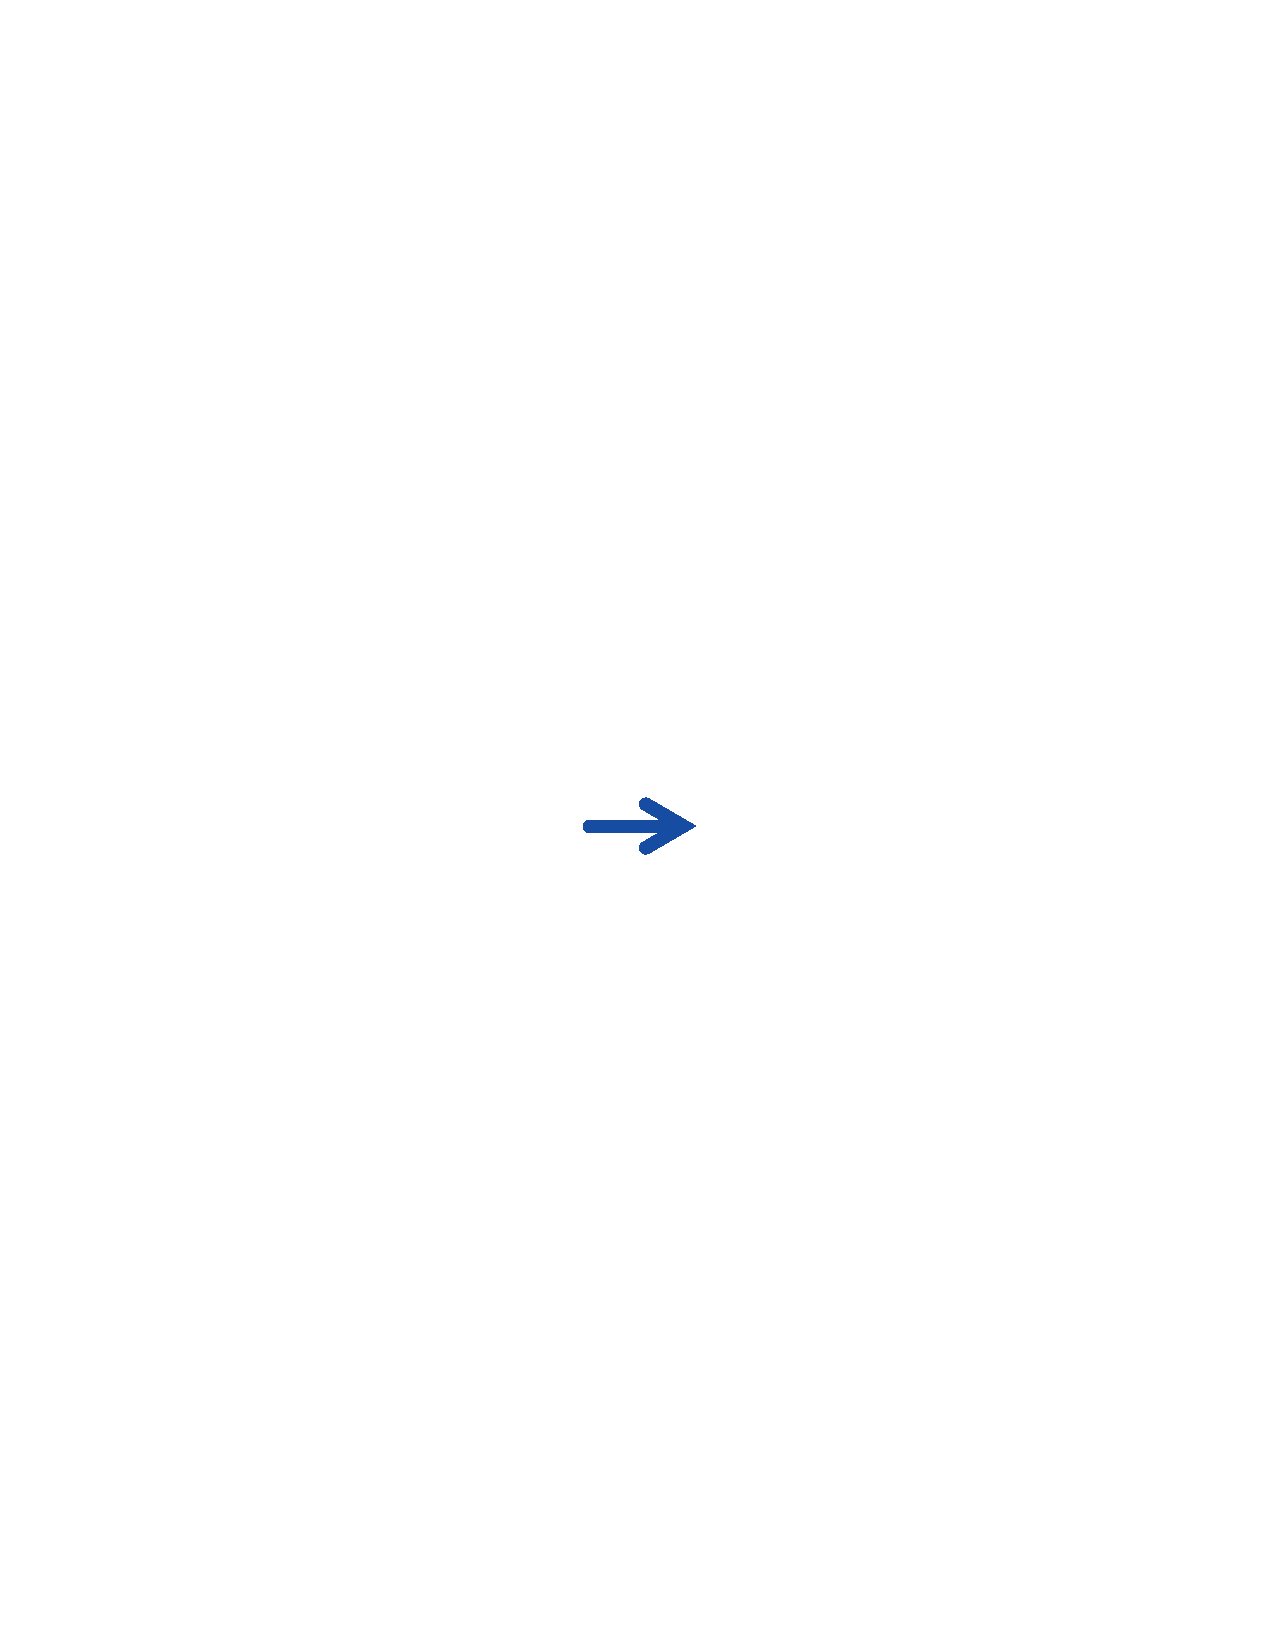
\includegraphics[width=40pt]{blue_arrow}}}
\end{picture}
\end{column}
\begin{column}{0.4\textwidth}
\begin{lstlisting}
void main() {
  bool p1, p2;

  p1=TRUE;
  p2=TRUE;

  while(p2) {
    p1= @p1 ? FALSE : *@;
    p2= @!p2@;
  }
}
\end{lstlisting}
\onslide<1-2| handout:0>{\begin{picture}(0,0)
\put(-15,0){\color{white}\rule{150pt}{155pt}}
\end{picture}}
\end{column}
\end{columns}

\hspace{0.1cm} C Program
\onslide<2->{\hspace{1.2cm} Predicates}
\onslide<3->{\hspace{1.5cm} Boolean Program}\\
\onslide<4->{\hspace{.8\textwidth}\color{ta3skyblue}Minimal?}

\end{frame}

% ------------------------------------------------------------------------
% ------------------------------------------------------------------------
% ------------------------------------------------------------------------

\subsection{Predicate Images}

\begin{frame}
\frametitle{Predicate Images}

Reminder:
\[ \mathit{Image}(X) = \{ s' \in S \,|\, \exists s\in X.\, T(s,s') \} \]
\vfill

We need
%
\[ \widehat{\mathit{Image}}(\hat X) = \{ \hat s' \in \hat S \,|\,
\exists \hat s \in \hat X.\, \hat T(\hat s,\hat s') \} \]
\vfill

$\widehat{\mathit{Image}}(\hat X)$ is equivalent to
%
\[ \{ \hat s, \hat s' \in \hat S^2 \,|\, \exists s,s' \in S^2.\,
\alpha(s)=\hat s \land \alpha(s')=\hat s' \land T(s,s') \} \]
%
This is called the \alert{predicate image} of $T$.

\end{frame}

% ------------------------------------------------------------------------
% ------------------------------------------------------------------------
% ------------------------------------------------------------------------

\begin{frame}
\frametitle{Enumeration}

\begin{itemize}
\item Let's take existential abstraction seriously
\vfill

\item Basic idea: with $n$ predicates, there are $2^n\cdot 2^n$
possible abstract transitions
\vfill

\item Let's just check them!
\end{itemize}

\end{frame}

% ------------------------------------------------------------------------
% ------------------------------------------------------------------------
% ------------------------------------------------------------------------

\begin{frame}
\frametitle{Enumeration: Example}

\begin{center}
\begin{tikzpicture}
%
% Predicates
%
\draw (2,8.2) node {\scriptsize Predicates};
\fill[gray!20] (0,6) rectangle (4,8);
\draw (2,7) node
{$\begin{array}{rcl}
p_1 &\iff& i=1 \\
p_2 &\iff& i=2 \\
p_3 &\iff& \mathsf{even}(i) \\
\end{array}$};
\pause
%
% Basic Block
%
\draw(6,7.8) node {\scriptsize Basic Block};
\fill[tabutter!50] (5,6.5) rectangle (7,7.5);
\draw (6,7) node {\lstinline!i++;!};
\pause
%
% Formula
%
\draw (8,7) node {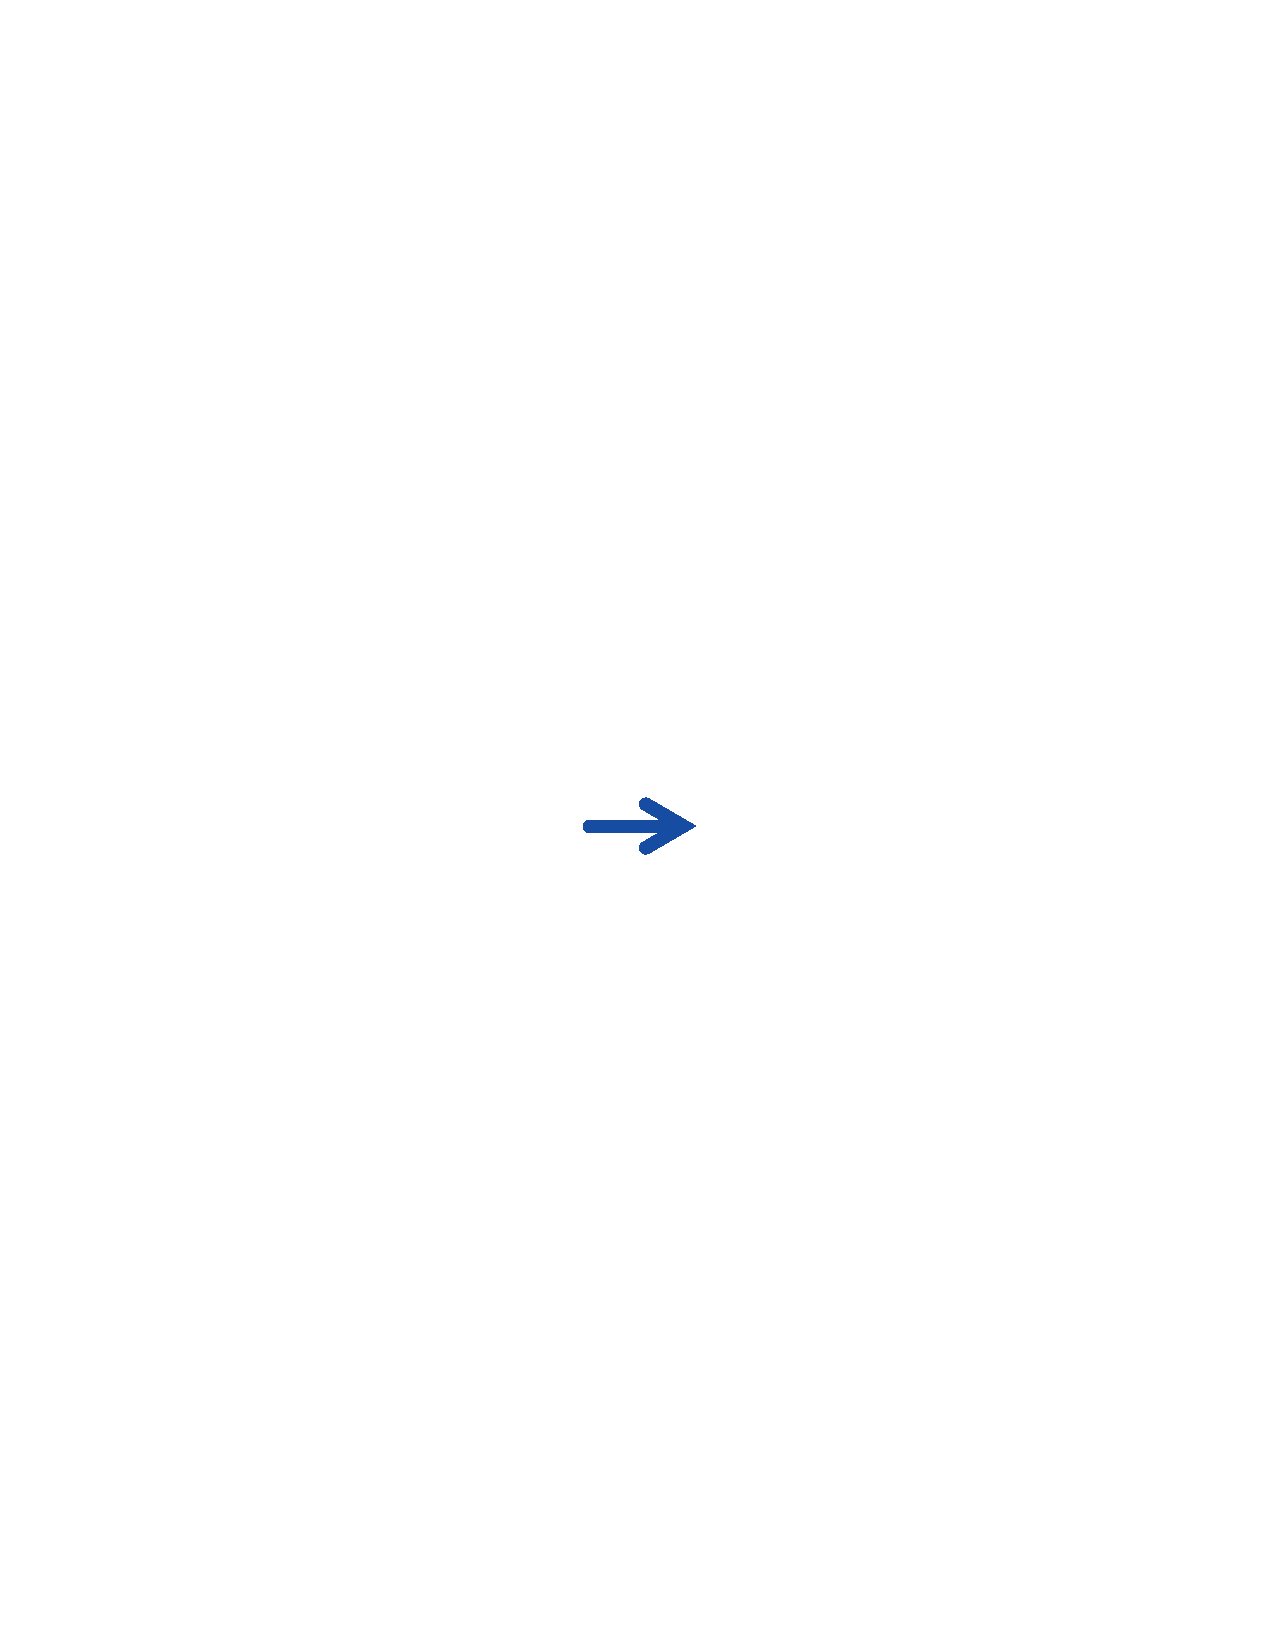
\includegraphics[width=1cm]{blue_arrow.pdf}};
\draw(10,7.8) node {\scriptsize $T$};
\fill[tabutter] (9,6.5) rectangle (11,7.5);
\draw (10,7) node {$i'=i+1$};
\pause
%
% Tables
%
\fill[taplum!20] (0,1) rectangle (2,5);
\draw[taplum] (0,1) rectangle (2,5);
\foreach \y in {1,1.5,...,5} \draw[taplum] (0,\y) -- (2,\y);
\draw[taplum] (.66,1) -- (.66,5);
\draw[taplum] (1.33,1) -- (1.33,5);
\draw (.33,5.2) node {$p_1$};
\draw (1,5.2) node {$p_2$};
\draw (1.66,5.2) node {$p_3$};
%
\draw (.33,4.75) node {$0$}; \draw (1,4.75) node {$0$}; \draw (1.66,4.75) node {$0$};
\draw (.33,4.25) node {$0$}; \draw (1,4.25) node {$0$}; \draw (1.66,4.25) node {$1$};
\draw (.33,3.75) node {$0$}; \draw (1,3.75) node {$1$}; \draw (1.66,3.75) node {$0$};
\draw (.33,3.25) node {$0$}; \draw (1,3.25) node {$1$}; \draw (1.66,3.25) node {$1$};
\draw (.33,2.75) node {$1$}; \draw (1,2.75) node {$0$}; \draw (1.66,2.75) node {$0$};
\draw (.33,2.25) node {$1$}; \draw (1,2.25) node {$0$}; \draw (1.66,2.25) node {$1$};
\draw (.33,1.75) node {$1$}; \draw (1,1.75) node {$1$}; \draw (1.66,1.75) node {$0$};
\draw (.33,1.25) node {$1$}; \draw (1,1.25) node {$1$}; \draw (1.66,1.25) node {$1$};
%
\fill[taplum!20] (4,1) rectangle (6,5);
\draw[taplum] (4,1) rectangle (6,5);
\foreach \y in {1,1.5,...,5} \draw[taplum] (4,\y) -- (6,\y);
\draw[taplum] (4.66,1) -- (4.66,5);
\draw[taplum] (5.33,1) -- (5.33,5);
\draw (4.33,5.3) node {$p_1'$};
\draw (5,5.3) node {$p_2'$};
\draw (5.66,5.3) node {$p_3'$};
%
\draw (4.33,4.75) node {$0$}; \draw (5,4.75) node {$0$}; \draw (5.66,4.75) node {$0$};
\draw (4.33,4.25) node {$0$}; \draw (5,4.25) node {$0$}; \draw (5.66,4.25) node {$1$};
\draw (4.33,3.75) node {$0$}; \draw (5,3.75) node {$1$}; \draw (5.66,3.75) node {$0$};
\draw (4.33,3.25) node {$0$}; \draw (5,3.25) node {$1$}; \draw (5.66,3.25) node {$1$};
\draw (4.33,2.75) node {$1$}; \draw (5,2.75) node {$0$}; \draw (5.66,2.75) node {$0$};
\draw (4.33,2.25) node {$1$}; \draw (5,2.25) node {$0$}; \draw (5.66,2.25) node {$1$};
\draw (4.33,1.75) node {$1$}; \draw (5,1.75) node {$1$}; \draw (5.66,1.75) node {$0$};
\draw (4.33,1.25) node {$1$}; \draw (5,1.25) node {$1$}; \draw (5.66,1.25) node {$1$};
%
\pause
%
% Arrow between tables
%
\onslide<5-6 | handout:0>{
\draw[->,thick] (2.2,4.75) -- node[ta3skyblue,font=\Large] {?} (3.8,4.75);
}
\onslide<7>{
\draw[->,thick] (2.2,4.75) -- node[ta3skyblue,font=\Large] {\myfail} (3.8,4.75);
}
\onslide<8 | handout:0>{
\draw[->,thick] (2.2,4.75) -- node[ta3skyblue,font=\Large] {?} (3.8,4.25);
}
\onslide<9>{
\draw[->,thick] (2.2,4.75) -- node[ta3skyblue,font=\Large] {\mycheck} (3.8,4.25);
}
\pause
%
% Query
%
\draw (9,5.3) node {\scriptsize Query to Solver};
\fill[taskyblue!20] (6.5,3) rectangle (11.5,5);
\onslide<6-7 | handout:0>{
\draw (9,4) node
{$\begin{array}{c}
i\not=1 \land i\not=2 \land \overline{\mathsf{even}(i)} \land\\
i'=i+1 \land \\
i'\not=1 \land i'\not=2 \land \overline{\mathsf{even}(i')}
\end{array}$};
}
\onslide<8-9>{
\draw (9,4) node
{$\begin{array}{c}
i\not=1 \land i\not=2 \land \overline{\mathsf{even}(i)} \land\\
i'=i+1 \land \\
i'\not=1 \land i'\not=2 \land \mathsf{even}(i')
\end{array}$};
}
%
% And so on
%
\onslide<10>{\draw (9,2) node {\ldots and so on \ldots};}
\end{tikzpicture}
\end{center}

\end{frame}

% ------------------------------------------------------------------------
% ------------------------------------------------------------------------
% ------------------------------------------------------------------------

\begin{frame}
\frametitle{Predicate Images}

\begin{itemize}

\item[\myfail] Computing the minimal existential abstraction can be way too slow
\vfill

\item Use an over-approximation instead
\begin{itemize}
\item[\mycheck] Fast(er) to compute
\item[\myfail] But has additional transitions
\end{itemize}
\vfill

\item Examples:
\begin{itemize}
\item Cartesian approximation (SLAM)
\item FastAbs (SLAM)
\item Lazy abstraction (Blast)
\item Predicate partitioning (VCEGAR)
\end{itemize}
\end{itemize}

\end{frame}

% ------------------------------------------------------------------------
% ------------------------------------------------------------------------
% ------------------------------------------------------------------------

\section{Checking the Abstract Model}

\begin{frame}
\frametitle{Checking the Abstract Model}

\begin{center}
\includegraphics{cegar-3}
\end{center}

\end{frame}

% ------------------------------------------------------------------------
% ------------------------------------------------------------------------
% ------------------------------------------------------------------------

\begin{frame}
\frametitle{Checking the Abstract Model}

\begin{itemize}
\item No more integers!
\vfill

\item But:
\begin{itemize}
\item All control flow constructs, including function calls
\item (more) non-determinism
\end{itemize}
\vfill

\item[\mycheck] BDD-based model checking now scales
\end{itemize}

\end{frame}

% ------------------------------------------------------------------------
% ------------------------------------------------------------------------
% ------------------------------------------------------------------------

\subsection{Finite-State Model Checkers}

\begin{frame}[fragile]
\frametitle{Finite-State Model Checkers: SMV}

\begin{tikzpicture}
\draw (0,0) node {
\includegraphics[width=3cm]{images/gradient_box_yellow}};
\draw (-1.1,0) node {\huge\ding{172}};
\draw (0.2,0) node {Variables};
\end{tikzpicture}

\begin{lstlisting}[basicstyle=\footnotesize,morekeywords={VAR,boolean}]
VAR b0_argc_ge_1: boolean;          -- argc >= 1
VAR b1_argc_le_2147483646: boolean; -- argc <= 2147483646
VAR b2: boolean;                    -- argv[argc] == NULL
VAR b3_nmemb_ge_r: boolean;         -- nmemb >= r
VAR b4: boolean;                    -- p1 == &array[0]
VAR b5_i_ge_8: boolean;             -- i >= 8
VAR b6_i_ge_s: boolean;             -- i >= s
VAR b7: boolean;                    -- 1 + i >= 8
VAR b8: boolean;                    -- 1 + i >= s
VAR b9_s_gt_0: boolean;             -- s > 0
VAR b10_s_gt_1: boolean;            -- s > 1
...
\end{lstlisting}

\end{frame}

% ------------------------------------------------------------------------
% ------------------------------------------------------------------------
% ------------------------------------------------------------------------

\begin{frame}[fragile]
\frametitle{Finite-State Model Checkers: SMV}

\begin{tikzpicture}
\draw (0,0) node {
\includegraphics[width=3cm]{images/gradient_box_yellow}};
\draw (-1.1,0) node {\huge\ding{173}};
\draw (0.3,0) node {Control Flow};
\end{tikzpicture}

\begin{lstlisting}[basicstyle=\footnotesize,morekeywords={VAR,ASSIGN,case,esac,init}]
-- program counter: 56 is the "terminating" PC
VAR PC: 0..56;
ASSIGN init(PC):=0; -- initial PC

ASSIGN next(PC):=case
    PC=0: 1; -- other
    PC=1: 2; -- other
    . . .
    PC=19: case  -- goto (with guard)
      guard19: 26;
      1: 20;
    esac;
    . . .
\end{lstlisting}

\end{frame}

% ------------------------------------------------------------------------
% ------------------------------------------------------------------------
% ------------------------------------------------------------------------

\begin{frame}[fragile]
\frametitle{Finite-State Model Checkers: SMV}

\begin{tikzpicture}
\draw (0,0) node {
\includegraphics[width=3cm]{images/gradient_box_yellow}};
\draw (-1.1,0) node {\huge\ding{174}};
\draw (0.1,0) node {Data};
\end{tikzpicture}

\begin{lstlisting}[basicstyle=\footnotesize,morekeywords={TRANS,next}]
TRANS (PC=0) -> next(b0_argc_ge_1)=b0_argc_ge_1
              & next(b1_argc_le_213646)=b1_argc_le_21646
              & next(b2)=b2
              & (!b30 | b36)
              & (!b17 | !b30 | b42)
              & (!b30 | !b42 | b48)
              & (!b17 | !b30 | !b42 | b54)
              & (!b54 | b60)

TRANS (PC=1) -> next(b0_argc_ge_1)=b0_argc_ge_1
              & next(b1_argc_le_214646)=b1_argc_le_214746
              & next(b2)=b2
              & next(b3_nmemb_ge_r)=b3_nmemb_ge_r
              & next(b4)=b4
              & next(b5_i_ge_8)=b5_i_ge_8
              & next(b6_i_ge_s)=b6_i_ge_s
              . . .
\end{lstlisting}

\end{frame}

% ------------------------------------------------------------------------
% ------------------------------------------------------------------------
% ------------------------------------------------------------------------

\begin{frame}[fragile]
\frametitle{Finite-State Model Checkers: SMV}

\begin{tikzpicture}
\draw (0,0) node {
\includegraphics[width=3cm]{images/gradient_box_yellow}};
\draw (-1.1,0) node {\huge\ding{175}};
\draw (0.1,0) node {Property};
\end{tikzpicture}

\begin{lstlisting}[basicstyle=\footnotesize,morekeywords={SPEC,AG}]
-- the specification

-- file main.c line 20 column 12
-- function c::very_buggy_function
SPEC AG ((PC=51) -> !b23)
\end{lstlisting}

\end{frame}

% ------------------------------------------------------------------------
% ------------------------------------------------------------------------
% ------------------------------------------------------------------------

\begin{frame}
\frametitle{Finite-State Model Checkers: SMV}

\begin{itemize}
\item If the property holds, we can terminate
\vfill

\item If the property fails, SMV generates a
{\color{ta3chameleon}counterexample}
with an assignment for all variables, including the PC

\end{itemize}

\end{frame}

% ------------------------------------------------------------------------
% ------------------------------------------------------------------------
% ------------------------------------------------------------------------

\subsection{Model Checkers for Pushdown Systems}

% ------------------------------------------------------------------------
% ------------------------------------------------------------------------
% ------------------------------------------------------------------------

\section{Simulating the Counterexample}

\begin{frame}
\frametitle{Simulating the Counterexample}

\begin{center}
\includegraphics{cegar-4}
\end{center}

\end{frame}

% ------------------------------------------------------------------------
% ------------------------------------------------------------------------
% ------------------------------------------------------------------------

\subsection{Lazy Abstraction}

\begin{frame}
\frametitle{Lazy Abstraction}

\begin{itemize}
\item The progress guarantee is only valid if the minimal existential
abstraction is used.
\vfill

\item Thus, distinguish \alert{spurious transitions} from \alert{spurious prefixes}.
\vfill

\item Refine spurious transitions separately to obtain minimal existential
abstraction

\item SLAM: {\tt Constrain}

\end{itemize}

\end{frame}

% ------------------------------------------------------------------------
% ------------------------------------------------------------------------
% ------------------------------------------------------------------------

\begin{frame}
\frametitle{Lazy Abstraction}

\begin{itemize}
\item One more observation:\\
each iteration only
{\color{ta3chameleon}causes only minor changes} in the abstract model
\vfill

\item Thus, use ``incremental Model Checker'', which
{\color{ta3skyblue}retains
the set of reachable states between iterations} (BLAST)

\end{itemize}

\end{frame}

% ------------------------------------------------------------------------
% ------------------------------------------------------------------------
% ------------------------------------------------------------------------

\subsection{Simulating Prefixes}

\lstset{language=C,morekeywords={bool}}

\newlength{\vvdist}
\setlength{\vvdist}{.6cm}

\begin{frame}[fragile]
\frametitle{Example Simulation}

\begin{columns}

\begin{column}{.3\textwidth}
\begin{tikzpicture}
\draw (0.0cm,9\vvdist) node[right] {\lstinline!int main() {!};
\draw (0.7cm,8\vvdist) node[right] {\lstinline!int x, y;!};
\draw (0.7cm,7\vvdist) node[right] {\lstinline!y=1;!};
\draw (0.7cm,6\vvdist) node[right] {\lstinline!x=1;!};
\draw (0.7cm,5\vvdist) node[right] {\lstinline!if(y>x)!};
\draw (1.4cm,4\vvdist) node[right] {\lstinline!y--;!};
\draw (0.7cm,3\vvdist) node[right] {\lstinline!else!};
\draw (1.4cm,2\vvdist) node[right] {\lstinline!y++;!};
\draw (0.7cm,1\vvdist) node[right] {\lstinline!assert(y>x);!};
\draw (0.0cm,0\vvdist) node[right] {\lstinline!}!};
\end{tikzpicture}
\end{column}

\begin{column}{.1\textwidth}
\begin{center}
Predicate: \alert{\lstinline!y>x!}


\includegraphics[width=\textwidth]{images/arrow}
\end{center}
\end{column}

\begin{column}{.4\textwidth}
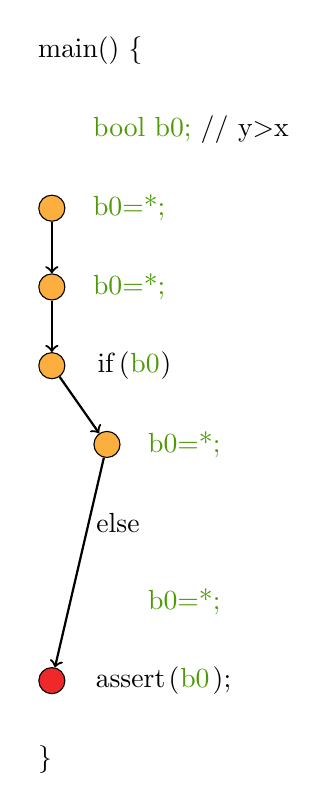
\begin{tikzpicture}
\draw (0.0cm,9\vvdist) node[right] {\lstinline!main() {!};
\draw (0.7cm,8\vvdist) node[right] {{\color{ta3chameleon}bool b0;} \lstinline!// y>x!};
\draw (0.7cm,7\vvdist) node[right] {{\color{ta3chameleon}b0=*;}};
\draw (0.7cm,6\vvdist) node[right] {{\color{ta3chameleon}b0=*;}};
\draw (0.7cm,5\vvdist) node[right] {\lstinline!if(!{\color{ta3chameleon}b0}\lstinline!)!};
\draw (1.4cm,4\vvdist) node[right] {{\color{ta3chameleon}b0=*;}};
\draw (0.7cm,3\vvdist) node[right] {\lstinline!else!};
\draw (1.4cm,2\vvdist) node[right] {{\color{ta3chameleon}b0=*;}};
\draw (0.7cm,1\vvdist) node[right] {\lstinline!assert(!{\color{ta3chameleon}b0}\lstinline!);!};
\draw (0.0cm,0\vvdist) node[right] {\lstinline!}!};
\pause
\tikzstyle{state}=[circle,draw=black,fill=taorange,minimum size=1.5mm]
\draw (0.3cm,7\vvdist) node[state] (s0) {};
\draw (0.3cm,6\vvdist) node[state] (s1) {};
\draw (0.3cm,5\vvdist) node[state] (s2) {};
\draw (1.0cm,4\vvdist) node[state] (s3) {};
\draw (0.3cm,1\vvdist) node[state,fill=tascarletred] (s4) {};
\draw[->,thick] (s0) -- (s1);
\draw[->,thick] (s1) -- (s2);
\draw[->,thick] (s2) -- (s3);
\draw[->,thick] (s3) -- (s4);
\end{tikzpicture}
\end{column}

\end{columns}

\end{frame}

% ------------------------------------------------------------------------
% ------------------------------------------------------------------------
% ------------------------------------------------------------------------

\begin{frame}[fragile]
\frametitle{Example Simulation}

\begin{columns}

\begin{column}{.3\textwidth}
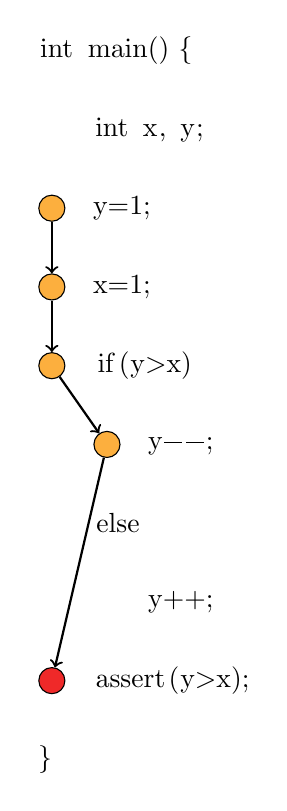
\begin{tikzpicture}
\draw (0.0cm,9\vvdist) node[right] {\lstinline!int main() {!};
\draw (0.7cm,8\vvdist) node[right] {\lstinline!int x, y;!};
\draw (0.7cm,7\vvdist) node[right] {\lstinline!y=1;!};
\draw (0.7cm,6\vvdist) node[right] {\lstinline!x=1;!};
\draw (0.7cm,5\vvdist) node[right] {\lstinline!if(y>x)!};
\draw (1.4cm,4\vvdist) node[right] {\lstinline!y--;!};
\draw (0.7cm,3\vvdist) node[right] {\lstinline!else!};
\draw (1.4cm,2\vvdist) node[right] {\lstinline!y++;!};
\draw (0.7cm,1\vvdist) node[right] {\lstinline!assert(y>x);!};
\draw (0.0cm,0\vvdist) node[right] {\lstinline!}!};
\tikzstyle{state}=[circle,draw=black,fill=taorange,minimum size=1.5mm]
\draw (0.3cm,7\vvdist) node[state] (s0) {};
\draw (0.3cm,6\vvdist) node[state] (s1) {};
\draw (0.3cm,5\vvdist) node[state] (s2) {};
\draw (1.0cm,4\vvdist) node[state] (s3) {};
\draw (0.3cm,1\vvdist) node[state,fill=tascarletred] (s4) {};
\draw[->,thick] (s0) -- (s1);
\draw[->,thick] (s1) -- (s2);
\draw[->,thick] (s2) -- (s3);
\draw[->,thick] (s3) -- (s4);
\end{tikzpicture}
\end{column}

\begin{column}{.1\textwidth}
\end{column}

\begin{column}{.4\textwidth}
\pause
We now do a path test,
so convert to SSA.
\end{column}

\end{columns}

\end{frame}

% ------------------------------------------------------------------------
% ------------------------------------------------------------------------
% ------------------------------------------------------------------------

\begin{frame}[fragile]
\frametitle{Example Simulation}

\begin{columns}

\begin{column}{.3\textwidth}
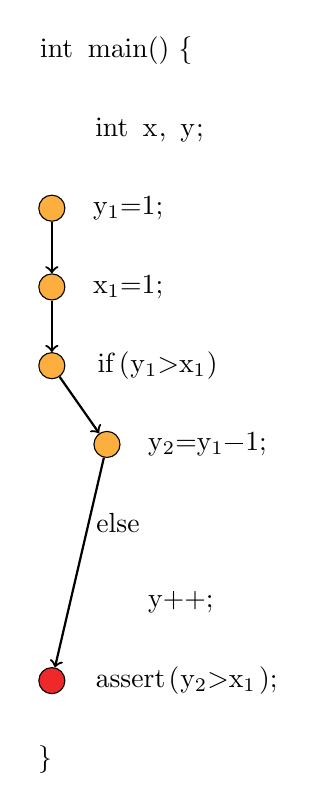
\begin{tikzpicture}
\draw (0.0cm,9\vvdist) node[right] {\lstinline!int main() {!};
\draw (0.7cm,8\vvdist) node[right] {\lstinline!int x, y;!};
\draw (0.7cm,7\vvdist) node[right] {\lstinline!y!\alert{$_1$}\lstinline!=1;!};
\draw (0.7cm,6\vvdist) node[right] {\lstinline!x!\alert{$_1$}\lstinline!=1;!};
\draw (0.7cm,5\vvdist) node[right] {\lstinline!if(y!\alert{$_1$}\lstinline!>x!\alert{$_1$}\lstinline!)!};
\draw (1.4cm,4\vvdist) node[right] {\lstinline!y!\alert{$_2$}\lstinline!=y!\alert{$_1$}\lstinline!-1;!};
\draw (0.7cm,3\vvdist) node[right] {\lstinline!else!};
\draw (1.4cm,2\vvdist) node[right] {\lstinline!y++;!};
\draw (0.7cm,1\vvdist) node[right] {\lstinline!assert(y!\alert{$_2$}\lstinline!>x!\alert{$_1$}\lstinline!);!};
\draw (0.0cm,0\vvdist) node[right] {\lstinline!}!};
\tikzstyle{state}=[circle,draw=black,fill=taorange,minimum size=1.5mm]
\draw (0.3cm,7\vvdist) node[state] (s0) {};
\draw (0.3cm,6\vvdist) node[state] (s1) {};
\draw (0.3cm,5\vvdist) node[state] (s2) {};
\draw (1.0cm,4\vvdist) node[state] (s3) {};
\draw (0.3cm,1\vvdist) node[state,fill=tascarletred] (s4) {};
\draw[->,thick] (s0) -- (s1);
\draw[->,thick] (s1) -- (s2);
\draw[->,thick] (s2) -- (s3);
\draw[->,thick] (s3) -- (s4);
\end{tikzpicture}
\end{column}

\begin{column}{.1\textwidth}
\pause

\includegraphics[width=\textwidth]{images/arrow}
\end{column}

\begin{column}{.3\textwidth}
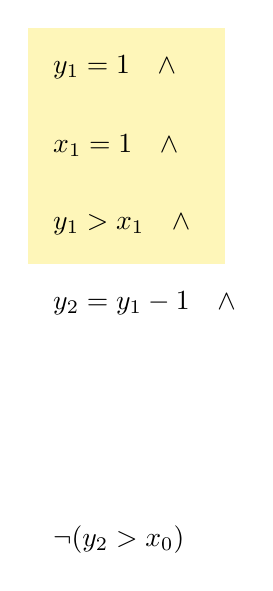
\begin{tikzpicture}
\onslide<3>{
\fill[tabutter!40] (0.5cm,4.5\vvdist) rectangle (3cm,7.5\vvdist);
}
\draw (0.7cm,7\vvdist) node[right] {$y_1=1 \quad \land$};
\draw (0.7cm,6\vvdist) node[right] {$x_1=1 \quad \land$};
\draw (0.7cm,5\vvdist) node[right] {$y_1>x_1 \quad \land$};
\draw (0.7cm,4\vvdist) node[right] {$y_2=y_1-1 \quad \land$};
\draw (0.7cm,1\vvdist) node[right] {$\neg (y_2>x_0)$};
\end{tikzpicture}
\pause 
This is UNSAT, so $\hat\pi$ is spurious.
\end{column}

\end{columns}

\end{frame}

% ------------------------------------------------------------------------
% ------------------------------------------------------------------------
% ------------------------------------------------------------------------

\section{Refining the Abstraction}

\begin{frame}
\frametitle{Refining the Abstraction}

\begin{center}
\includegraphics{cegar-5}
\end{center}

\end{frame}

% ------------------------------------------------------------------------
% ------------------------------------------------------------------------
% ------------------------------------------------------------------------

\subsection{Predicate Refinement using Proofs}

\begin{frame}[fragile]
\frametitle{Manual Proof!}

\begin{columns}
\begin{column}{.6\textwidth}
\lstinline!int main() {!\\
\hspace*{0.7cm} \lstinline!int x, y;!\\[0.5ex]
\hspace*{0.7cm} \lstinline!y=1;!\\[0.5ex]
\hspace*{0.7cm} \onslide<2->{{\color{red}$\{y=1\}$}}\\[0.5ex]
\hspace*{0.7cm} \lstinline!x=1;!\\[0.5ex]
\hspace*{0.7cm} \onslide<3->{{\color{red}$\{x=1 \wedge y=1\}$}}\\[0.5ex]
\hspace*{0.7cm} \lstinline!if(y>x)!\\
\hspace*{1.4cm} \lstinline!y--;!\\
\hspace*{0.7cm} \lstinline!else!\\
\hspace*{1.4cm} \onslide<4->{{\color{red}$\{x=1 \wedge y=1 \wedge \neg y>x\}$}}\\[1ex]
\hspace*{1.4cm} \lstinline!y++;!\\[1ex]
\hspace*{0.7cm} \onslide<5->{{\color{red}$\{x=1 \wedge y=2 \wedge y>x\}$}}\\[1ex]
\hspace*{0.7cm} \lstinline!assert(y>x);!\\
\lstinline!}!
\end{column}
\begin{column}{.3\textwidth}
\onslide<5->{This proof uses \alert{strongest post-conditions}
}
\end{column}
\end{columns}

\end{frame}

% ------------------------------------------------------------------------
% ------------------------------------------------------------------------
% ------------------------------------------------------------------------

\begin{frame}[fragile]
\frametitle{An Alternative Proof}

\begin{columns}
\begin{column}{.5\textwidth}
\lstinline!int main() {!\\
\hspace*{0.7cm} \lstinline!int x, y;!\\[0.5ex]
\hspace*{0.7cm} \lstinline!y=1;!\\[0.5ex]
\hspace*{0.7cm} {\onslide<5->{\color{red}$\{\neg y>1 \implies y+1>1\}$}}\\[0.5ex]
\hspace*{0.7cm} \lstinline!x=1;!\\[0.5ex]
\hspace*{0.7cm} \onslide<4->{{\color{red}$\{\neg y>x \implies y+1>x\}$}}\\[0.5ex]
\hspace*{0.7cm} \lstinline!if(y>x)!\\
\hspace*{1.4cm} \lstinline!y--;!\\
\hspace*{0.7cm} \lstinline!else!\\
\hspace*{1.4cm} \onslide<3->{{\color{red}$\{y+1>x\}$}}\\[1ex]
\hspace*{1.4cm} \lstinline!y++;!\\[1ex]
\hspace*{0.7cm} \onslide<2->{{\color{red}$\{y>x\}$}}\\[1ex]
\hspace*{0.7cm} \lstinline!assert(y>x);!\\
\lstinline!}!
\end{column}

\begin{column}{.5\textwidth}
\onslide<6->{We are using weakest pre-conditions here\\[2ex]

\begin{scriptsize}
$wp(x\texttt{:=}E, P)=P[x/E]$\\[1ex]
$wp(S\texttt{;}T, Q) = wp(S, wp(T, Q))$\\[1ex]
$wp(\texttt{if(}c\texttt{) } A \texttt{ else } B, P) =$\\
\hspace*{2cm}$(B\implies wp(A, P))\wedge$\\
\hspace*{2cm}$(\neg B\implies wp(B, P))$
\end{scriptsize}\\[2ex]

The proof for the "true" branch is missing
}
\end{column}
\end{columns}

\end{frame}

% ------------------------------------------------------------------------
% ------------------------------------------------------------------------
% ------------------------------------------------------------------------

\begin{frame}
\frametitle{Refinement Algorithms}

\underline{Using WP}

\begin{enumerate}
\item Start with failed guard $G$
\item Compute $wp(G)$ along the path
\end{enumerate}
\vfill

\underline{Using SP}

\begin{enumerate}
\item Start at beginning
\item Compute $sp(\ldots)$ along the path
\end{enumerate}
\vfill

\begin{itemize}
\item Both methods eliminate the trace
\item Advantages/disadvantages?
\end{itemize}

\end{frame}

% ------------------------------------------------------------------------
% ------------------------------------------------------------------------
% ------------------------------------------------------------------------

\subsection{Predicate Localization}

\lstset{language=C}

\begin{frame}[fragile]
\frametitle{Predicate Localization}

Example:
\vfill

\begin{center}
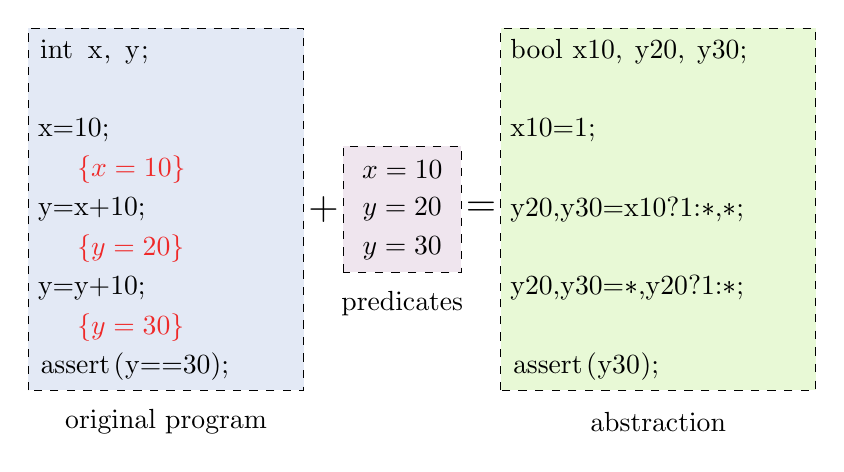
\begin{tikzpicture}

\fill[taskyblue!20!white] (0,-.3) rectangle (3.5,4.3);
\draw[dashed] (0,-.3) rectangle (3.5,4.3);
\draw (0,4) node [right] { \lstinline!int x, y;! };
\draw (0,3) node [right] { \lstinline!x=10;! };
\onslide<4->{\draw (.5,2.5) node [right] { \color{tascarletred}$\{x=10\}$ };}
\draw (0,2) node [right] { \lstinline!y=x+10;! };
\onslide<4->{\draw (.5,1.5) node [right] { \color{tascarletred}$\{y=20\}$ };}
\draw (0,1) node [right] { \lstinline!y=y+10;! };
\onslide<4->{\draw (.5,.5) node [right] { \color{tascarletred}$\{y=30\}$ };}
\draw (0,0) node [right] { \lstinline!assert(y==30);! };
\draw (1.75,-.7) node { original program };
\pause

\draw (3.75,2) node [font=\Large] { $+$ };

\fill[taplum!20!white] (4,1.2) rectangle (5.5,2.8);
\draw[dashed] (4,1.2) rectangle (5.5,2.8);
\draw (4.75,2.5) node { $x=10$ };
\draw (4.75,2.0) node { $y=20$ };
\draw (4.75,1.5) node { $y=30$ };
\draw (4.75,.8) node { predicates };
\pause

\draw (5.75,2) node [font=\Large] { $=$ };

\fill[tachameleon!20!white] (6,-.3) rectangle (10,4.3);
\draw[dashed] (6,-.3) rectangle (10,4.3);
\draw (6,4) node [right] { \lstinline!bool x10, y20, y30;! };
\draw (6,3) node [right] { \lstinline!x10=1;! };
\draw (6,2) node [right] { \lstinline!y20,y30=x10?1:*,*;! };
\draw (6,1) node [right] { \lstinline!y20,y30=*,y20?1:*;! };
\draw (6,0) node [right] { \lstinline!assert(y30);! };
\draw (8,-.7) node { abstraction };

\end{tikzpicture}
\end{center}

\begin{center}
\onslide<5>{
We really only want to track \alert{specific predicates} at each location!}
\end{center}

\end{frame}

% ------------------------------------------------------------------------
% ------------------------------------------------------------------------
% ------------------------------------------------------------------------

\begin{frame}
\frametitle{Predicate Localization}

\begin{itemize}
\item Track a \alert{separate set of predicates} for each location
\vfill

\item[\mycheck] Makes predicate image easier

\item[\mycheck] Makes simulation of transitions easier

\item[\mycheck] Makes the check of the abstract model easier

\end{itemize}

\end{frame}

% ------------------------------------------------------------------------
% ------------------------------------------------------------------------
% ------------------------------------------------------------------------

\subsection{Predicate Refinement with Craig Interpolation}

\begin{frame}
\frametitle{Predicate Refinement for Paths}

Recall the decision problem we build for simulating paths:
\vfill

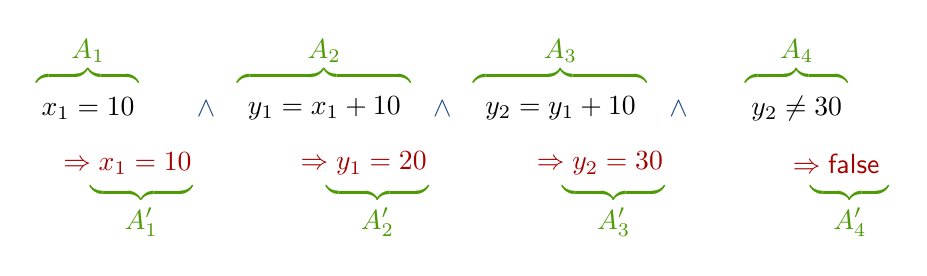
\begin{tikzpicture}

\draw (0,.7) node { $x_1=10$ };
\draw (1.5,.7) node { \color{ta3skyblue}$\land$ };
\draw (3,.7) node { $y_1=x_1+10$ };
\draw (4.5,.7) node { \color{ta3skyblue}$\land$ };
\draw (6,.7) node { $y_2=y_1+10$ };
\draw (7.5,.7) node { \color{ta3skyblue}$\land$ };
\draw (9,.7) node { $y_2\not=30$ };
\pause
\draw (0.5,0) node { \color{ta3scarletred}$\implies x_1=10$ };
\pause
\draw (3.5,0) node { \color{ta3scarletred}$\implies y_1=20$ };
\pause
\draw (6.5,0) node { \color{ta3scarletred}$\implies y_2=30$ };
\pause
\draw (9.5,0) node { \color{ta3scarletred}$\implies \textsf{false}$ };
\pause
\draw (0,1.3) node { \color{ta3chameleon}$\overbrace{\hspace{1.3cm}}^{\displaystyle A_1}$ };
\draw (3,1.3) node { \color{ta3chameleon}$\overbrace{\hspace{2.2cm}}^{\displaystyle A_2}$ };
\draw (6,1.3) node { \color{ta3chameleon}$\overbrace{\hspace{2.2cm}}^{\displaystyle A_3}$ };
\draw (9,1.3) node { \color{ta3chameleon}$\overbrace{\hspace{1.3cm}}^{\displaystyle A_4}$ };
\pause
\draw (0.5,-.6) node { \color{ta3chameleon}\quad$\underbrace{\hspace{1.3cm}}_{\displaystyle A'_1}$ };
\draw (3.5,-.6) node { \color{ta3chameleon}\quad$\underbrace{\hspace{1.3cm}}_{\displaystyle A'_2}$ };
\draw (6.5,-.6) node { \color{ta3chameleon}\quad$\underbrace{\hspace{1.3cm}}_{\displaystyle A'_3}$ };
\draw (9.5,-.6) node { \color{ta3chameleon}\quad$\underbrace{\hspace{1.0cm}}_{\displaystyle A'_4}$ };
\end{tikzpicture}

\end{frame}

% ------------------------------------------------------------------------
% ------------------------------------------------------------------------
% ------------------------------------------------------------------------

\begin{frame}
\frametitle{Predicate Refinement for Paths}

For a path with $n$ steps:

\begin{center}
\begin{tikzpicture}
\draw (0,.5) node { $A_1$ };
\draw (2,.5) node { $A_2$ };
\draw (4,.5) node { $A_3$ };
\draw (6,.5) node { $\ldots$ };
\draw (8,.5) node { $A_n$ };
\draw[dashed] (1,0) -- (1,1);
\draw[dashed] (3,0) -- (3,1);
\draw[dashed] (5,0) -- (5,1);
\draw[dashed] (7,0) -- (7,1);
\draw (-1,-.5) node { \color{ta3chameleon}\textsf{true} };
\draw (.6,-.5) node { $\implies$ };
\draw (1,-.5) node { \color{ta3chameleon}$A'_1$ };
\draw (2.6,-.5) node { $\implies$ };
\draw (3,-.5) node { \color{ta3chameleon}$A'_2$ };
\draw (4.6,-.5) node { $\implies$ };
\draw (5,-.5) node { \color{ta3chameleon}$A'_3$ };
\draw (6.4,-.5) node { $\implies$ };
\draw (7,-.5) node { \color{ta3chameleon}$A'_{n-1}$ };
\draw (8.4,-.5) node { $\implies$ };
\draw (9,-.5) node { \color{ta3chameleon}\textsf{false} };
\end{tikzpicture}
\end{center}
\pause

\begin{itemize}
\item Given $A_1,\ldots,A_n$ with $\bigwedge_i A_i = \textsf{false}$
\item $A'_0=\textsf{true}$ and $A'_n=\textsf{false}$
\item $(A'_{i-1}\land A_i)\implies A'_i$ for $i \in \{1, \ldots, n\}$
\pause
\item Finally, $\mathit{Vars}(A'_i) \subseteq
(\mathit{Vars}(A_1\ldots A_i)\cap
\mathit{Vars}(A_{i+1}\ldots A_n))$
\end{itemize}

\end{frame}

% ------------------------------------------------------------------------
% ------------------------------------------------------------------------
% ------------------------------------------------------------------------

\begin{frame}
\frametitle{Predicate Refinement for Paths}

Special case $n=2$:

\begin{itemize}
\item $A \land B = \textsf{false}$
\item $A \implies A'$
\item $A' \land B = \textsf{false}$
\item $\mathit{Vars}(A') \subseteq
(\mathit{Vars}(A)\cap\mathit{Vars}(B))$
\end{itemize}
\vfill

\pause
\begin{center}
\colorbox{tabutter!30}{\begin{minipage}{.7\textwidth}
\alert{W.~Craig's Interpolation theorem} (1957):\\
such an $A'$ exists for any first-order,\\
inconsistent $A$ and $B$.
\end{minipage}}
\end{center}

\end{frame}

% ------------------------------------------------------------------------
% ------------------------------------------------------------------------
% ------------------------------------------------------------------------

\begin{frame}
\frametitle{Predicate Refinement with Craig Interpolants}

\begin{itemize}

\item[\mycheck] For propositional logic, a propositional Craig Interpolant
can be extracted from a resolution proof ($\rightarrow$ SAT!)
in linear time
\vfill

\item[\mycheck] Interpolating solvers available for {\color{ta3skyblue}linear
arithmetic over the reals} and {\color{ta3skyblue}integer difference logic}
with uninterpreted functions
\vfill

\item[\myfail] Not possible for every fragment of FOL:
\[ x = 2y \quad\mbox{and}\quad x=2z+1 \qquad\mbox{ with } x,y,z \in \mathds{Z}\]
\pause
%
The interpolant is ``$x$ is even''

\end{itemize}

\end{frame}

% ------------------------------------------------------------------------
% ------------------------------------------------------------------------
% ------------------------------------------------------------------------

\begin{frame}
\frametitle{Craig Interpolation for Linear Inequalities}

\[ \frac{\displaystyle 0 \le x \quad 0 \le y}{\displaystyle 0 \le c_1 x + c_2 y}
\quad \mbox{with } 0 \le c_1,c_2 \]
\vfill

\begin{itemize}

\item ``Cutting-planes''
\vfill

\item Naturally arise in Fourier-Motzkin or Simplex

\end{itemize}

\end{frame}

% ------------------------------------------------------------------------
% ------------------------------------------------------------------------
% ------------------------------------------------------------------------

\begin{frame}
\frametitle{Example}

\begin{center}
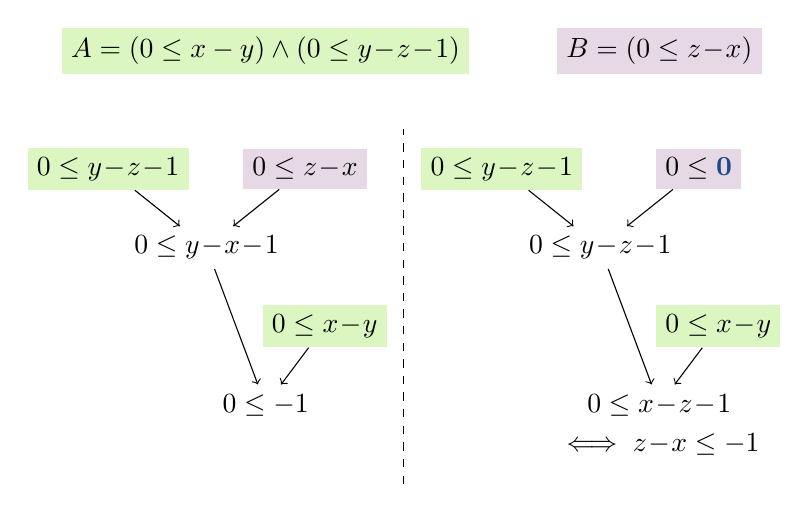
\begin{tikzpicture}
\draw (2,7.5) node[rectangle,fill=tachameleon!30] { $A = (0 \le \alert{x}-y) \land (0 \le y\!-\!\alert{z}\!-\!1)$ };
\draw (7,7.5) node[rectangle,fill=taplum!30] { $B = (0 \le \alert{z}\!-\!\alert{x})$ };
\pause
\draw (0,6) node[rectangle,fill=tachameleon!30] (n1) { $0\le y\!-\!\alert{z}\!-\!1$ };
\draw (2.5,6) node[rectangle,fill=taplum!30] (n2) { $0\le \alert{z}\!-\!\alert{x}$ };
\pause
\draw (1.25,5) node (n3) { $0 \le y\!-\!\alert{x}\!-\!1$ };
\draw[->] (n1) -- (n3);
\draw[->] (n2) -- (n3);
\pause
\draw (2.75,4) node[rectangle,fill=tachameleon!30] (n4) { $0 \le \alert{x}\!-\!y$ };
\draw (2,3) node (n5) { $0 \le -1$ };
\draw[->] (n3) -- (n5);
\draw[->] (n4) -- (n5);
%
\pause
\draw[dashed] (3.75,2) -- (3.75,6.5);
\draw (5,6) node[rectangle,fill=tachameleon!30] (m1) { $0\le y\!-\!\alert{z}\!-\!1$ };
\draw (7.5,6) node[rectangle,fill=taplum!30] (m2) { $0\le {\bf\color{ta3skyblue} 0}$ };
\draw (6.25,5) node (m3) { $0 \le y\!-\!\alert{z}\!-\!1$ };
\draw[->] (m1) -- (m3);
\draw[->] (m2) -- (m3);
\draw (7.75,4) node[rectangle,fill=tachameleon!30] (m4) { $0 \le \alert{x}\!-\!y$ };
\draw (7,3) node (m5) { $0 \le \alert{x}\!-\!\alert{z}\!-\!1$ };
\draw[->] (m3) -- (m5);
\draw[->] (m4) -- (m5);
\pause
\draw (7,2.5) node (m6) { $\iff \alert{z}\!-\!\alert{x} \le -1$ };
\end{tikzpicture}
\end{center}
\vfill
\onslide<7->{
Just sum the inequalities from
\colorbox{tachameleon!30}{$A$}, and you get an interpolant!
}

\end{frame}

% ------------------------------------------------------------------------
% ------------------------------------------------------------------------
% ------------------------------------------------------------------------

\begin{frame}[fragile]
\frametitle{Approximating Loop Invariants: SP}

\begin{columns}
\begin{column}{.3\textwidth}
\begin{lstlisting}
int x, y;

x=y=0;

while(x!=10) {
  x++;
  y++;
}

assert(y==10);
\end{lstlisting}
\end{column}
\begin{column}{.6\textwidth}
The SP refinement results in
%
\[ \begin{array}{lll}
sp(\lstinline!x=y=0!, \textsf{true}) &=& x=0 \land y=0 \\
\pause
sp(\lstinline!x++; y++!, \ldots) &=& x=1 \land y=1 \\
\pause
sp(\lstinline!x++; y++!, \ldots) &=& x=2 \land y=2 \\
\pause
sp(\lstinline!x++; y++!, \ldots) &=& x=3 \land y=3 \\
\ldots
\end{array} \]
\end{column}
\end{columns}
\vfill

\myfail{} 10 iterations required to prove the property.\\
\myfail{} It won't work if we replace $10$ by $n$.

\end{frame}

% ------------------------------------------------------------------------
% ------------------------------------------------------------------------
% ------------------------------------------------------------------------

\begin{frame}[fragile]
\frametitle{Approximating Loop Invariants: WP}

\begin{columns}
\begin{column}{.3\textwidth}
\begin{lstlisting}
int x, y;

x=y=0;

while(x!=10) {
  x++;
  y++;
}

assert(y==10);
\end{lstlisting}
\end{column}
\begin{column}{.6\textwidth}
The WP refinement results in
%
\[ \begin{array}{lll}
wp(\lstinline!x==10!, y\not=10) &=& y\not=10 \land x=10 \\
\pause
wp(\lstinline!x++; y++!, \ldots) &=& y\not=9 \land x=9 \\
\pause
wp(\lstinline!x++; y++!, \ldots) &=& y\not=8 \land x=8 \\
\pause
wp(\lstinline!x++; y++!, \ldots) &=& y\not=7 \land x=7 \\
\pause
\ldots
\end{array} \]
\end{column}
\end{columns}
\vfill

\myfail{} Also requires 10 iterations.\\
\myfail{} It won't work if we replace $10$ by $n$.

\end{frame}

% ------------------------------------------------------------------------
% ------------------------------------------------------------------------
% ------------------------------------------------------------------------

\newlength{\uxdist}
\setlength{\uxdist}{2.3cm}

\begin{frame}[fragile]
\frametitle{What do we really need?}

Consider an SSA-unwinding with $3$ loop iterations:
\vfill

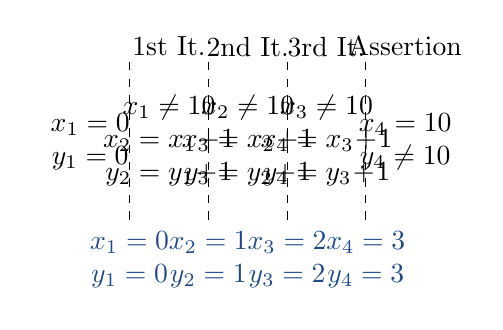
\begin{tikzpicture}
\draw (0\uxdist,0cm) node {$\begin{array}{c}x_1=0\\y_1=0\end{array}$};
\pause
%
\draw[dashed] (0.5\uxdist,-1cm) -- (0.5\uxdist,1cm);
\draw (1\uxdist,0cm) node {$\begin{array}{c}x_1\not=10\\x_2=x_1\!+\!1\\y_2=y_1\!+\!1\end{array}$};
\draw (1\uxdist,1.2cm) node {1st It.};
\pause
%
\draw[dashed] (1.5\uxdist,-1cm) -- (1.5\uxdist,1cm);
\draw (2\uxdist,0cm) node {$\begin{array}{c}x_2\not=10\\x_3=x_2\!+\!1\\y_3=y_2\!+\!1\end{array}$};
\draw (2\uxdist,1.2cm) node {2nd It.};
\pause
%
\draw[dashed] (2.5\uxdist,-1cm) -- (2.5\uxdist,1cm);
\draw (3\uxdist,0cm) node {$\begin{array}{c}x_3\not=10\\x_4=x_3\!+\!1\\y_4=y_3\!+\!1\end{array}$};
\draw (3\uxdist,1.2cm) node {3rd It.};
\pause
%
\draw[dashed] (3.5\uxdist,-1cm) -- (3.5\uxdist,1cm);
\draw (4\uxdist,0cm) node {$\begin{array}{c}x_4=10\\y_4\not=10\end{array}$};
\draw (4\uxdist,1.2cm) node {Assertion};
%
\pause
\draw (0.5\uxdist,-1.5cm) node[ta3skyblue] {$\begin{array}{c}x_1=0\\y_1=0\end{array}$};
\pause
\draw (1.5\uxdist,-1.5cm) node[ta3skyblue] {$\begin{array}{c}x_2=1\\y_2=1\end{array}$};
\pause
\draw (2.5\uxdist,-1.5cm) node[ta3skyblue] {$\begin{array}{c}x_3=2\\y_3=2\end{array}$};
\pause
\draw (3.5\uxdist,-1.5cm) node[ta3skyblue] {$\begin{array}{c}x_4=3\\y_4=3\end{array}$};
\end{tikzpicture}
\vfill

\onslide<10->{
{\myfail\color{ta3skyblue}\it This proof will produce the same predicates as SP.}
}

\end{frame}

% ------------------------------------------------------------------------
% ------------------------------------------------------------------------
% ------------------------------------------------------------------------

\begin{frame}[fragile]
\frametitle{Split Provers}

Idea:

\begin{center}
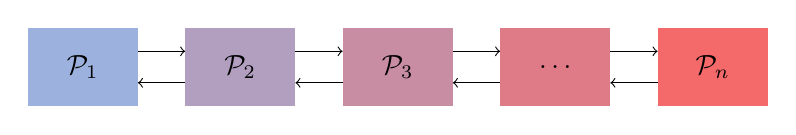
\begin{tikzpicture}
\fill[taskyblue!100!tascarletred!70] (0.3,0) rectangle (1.7,1);
\fill[taskyblue!075!tascarletred!70] (2.3,0) rectangle (3.7,1);
\fill[taskyblue!050!tascarletred!70] (4.3,0) rectangle (5.7,1);
\fill[taskyblue!025!tascarletred!70] (6.3,0) rectangle (7.7,1);
\fill[taskyblue!000!tascarletred!70] (8.3,0) rectangle (9.7,1);
\draw (1,.5) node { $\mathcal P_1$ };
\draw (3,.5) node { $\mathcal P_2$ };
\draw (5,.5) node { $\mathcal P_3$ };
\draw (7,.5) node { $\ldots$ };
\draw (9,.5) node { $\mathcal P_n$ };
\draw [->] (1.7,.7) -- (2.3,.7);
\draw [->] (3.7,.7) -- (4.3,.7);
\draw [->] (5.7,.7) -- (6.3,.7);
\draw [->] (7.7,.7) -- (8.3,.7);
\draw [<-] (1.7,.3) -- (2.3,.3);
\draw [<-] (3.7,.3) -- (4.3,.3);
\draw [<-] (5.7,.3) -- (6.3,.3);
\draw [<-] (7.7,.3) -- (8.3,.3);
\end{tikzpicture}
\end{center}

\begin{itemize}
\item Each prover $\mathcal P_i$ only knows $A_i$, but they exchange facts
\item We require that each prover only exchanges facts with common symbols
\item Plus, we restrict the facts exchanged to some language $\mathcal L$
\end{itemize}

\end{frame}

% ------------------------------------------------------------------------
% ------------------------------------------------------------------------
% ------------------------------------------------------------------------

\begin{frame}
\frametitle{Back to the Example}

Restriction to language $\mathcal L=$ ``no new constants'':
\vfill

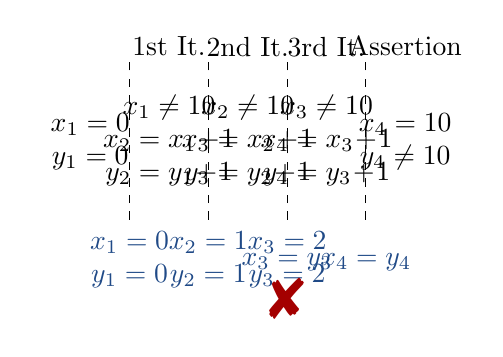
\begin{tikzpicture}
\draw (0\uxdist,0cm) node {$\begin{array}{c}x_1=0\\y_1=0\end{array}$};
%
\draw[dashed] (0.5\uxdist,-1cm) -- (0.5\uxdist,1cm);
\draw (1\uxdist,0cm) node {$\begin{array}{c}x_1\not=10\\x_2=x_1\!+\!1\\y_2=y_1\!+\!1\end{array}$};
\draw (1\uxdist,1.2cm) node {1st It.};
%
\draw[dashed] (1.5\uxdist,-1cm) -- (1.5\uxdist,1cm);
\draw (2\uxdist,0cm) node {$\begin{array}{c}x_2\not=10\\x_3=x_2\!+\!1\\y_3=y_2\!+\!1\end{array}$};
\draw (2\uxdist,1.2cm) node {2nd It.};
%
\draw[dashed] (2.5\uxdist,-1cm) -- (2.5\uxdist,1cm);
\draw (3\uxdist,0cm) node {$\begin{array}{c}x_3\not=10\\x_4=x_3\!+\!1\\y_4=y_3\!+\!1\end{array}$};
\draw (3\uxdist,1.2cm) node {3rd It.};
%
\draw[dashed] (3.5\uxdist,-1cm) -- (3.5\uxdist,1cm);
\draw (4\uxdist,0cm) node {$\begin{array}{c}x_4=10\\y_4\not=10\end{array}$};
\draw (4\uxdist,1.2cm) node {Assertion};
%
\pause
\draw (0.5\uxdist,-1.5cm) node[ta3skyblue] {$\begin{array}{c}x_1=0\\y_1=0\end{array}$};
\pause
\draw (1.5\uxdist,-1.5cm) node[ta3skyblue] {$\begin{array}{c}x_2=1\\y_2=1\end{array}$};
\onslide<4-5 | handout:0>{\draw (2.5\uxdist,-1.5cm) node[ta3skyblue] {$\begin{array}{c}x_3=2\\y_3=2\end{array}$};}
\onslide<5 | handout:0>{\draw (2.5\uxdist,-2cm) node[ta3scarletred] {\huge\myfail};}
\onslide<6->{\draw (2.5\uxdist,-1.5cm) node[ta3skyblue] {$\begin{array}{c}x_3=y_3\end{array}$};}
\onslide<7->{\draw (3.5\uxdist,-1.5cm) node[ta3skyblue] {$\begin{array}{c}x_4=y_4\end{array}$};}
\end{tikzpicture}

\end{frame}

% ------------------------------------------------------------------------
% ------------------------------------------------------------------------
% ------------------------------------------------------------------------

\begin{frame}
\frametitle{Invariants from Restricted Proofs}

\begin{itemize}

\item[\mycheck] The language restriction forces the solver to \alert{generalize}!
\vfill

\item Algorithm:
\end{itemize}

\begin{center}
\colorbox{tabutter!30}{\begin{minipage}{.7\textwidth}
\begin{itemize}
\item If the proof fails, increase $\mathcal L$!
\item If we fail to get a sufficiently strong invariant, increase $n$.
\end{itemize}
\end{minipage}}
\end{center}
\vfill

\begin{itemize}
\item[\mycheck] This does work if we replace $10$ by $n$!
\pause
\item[\bf\color{ta3skyblue}?] Which $\mathcal L_1, \mathcal L_2, \ldots$ is complete
for which programs?

\end{itemize}

\end{frame}

% ------------------------------------------------------------------------
% ------------------------------------------------------------------------
% ------------------------------------------------------------------------

\end{document}
